\chapter{BCS-BEC Crossover}
\label{chapter:bcs-bec-crossover}

In this Chapter, we investigate the spectral properties of the BCS-BEC crossover and present the main results of this work. A fully non-perturbative functional method~\cite{Horak2020} is applied to obtain spectral functions directly in real-time. We start with a simplified discussion of the normal phase and then present the general treatment in the superfluid phase. Numerical results of this work are compared to other approaches and existing results from the literature. In the end, the numerical framework is applied to describe recent experimental data from MIT~\cite{Mukherjee2019}.


\section{Normal phase}
\label{section:normal-phase}

Let us start with a discussion of the normal phase of the BCS-BEC crossover and introduce the basic concepts of the selfconsistent framework. As mentioned before, we are dealing with a balanced system in which the propagators of the $\uparrow$ and $\downarrow$ species are the same and we are left with only one fermion propagator $G_{\psi\psi^*} = G_{\psi_{\uparrow}\psi_{\uparrow}^*} = G_{\psi_{\downarrow}\psi_{\downarrow}^*}$. Since we are restricting ourselves to the normal phase, the gap parameter $\Delta$ is zero and the matrix propagator is diagonal. The Dyson-Schwinger equations for this system can be derived from the master DSE~\eqref{eq:DSE-general} by using the single-channel action in Eq.~\eqref{eq:single-channel-action}. Schematically, the fermion DSE reads
%
\begin{align}
	\label{eq:fermion-DSE}
	\Gamma^{(2)}_{\psi\psi^*} = S^{(2)}_{\psi\psi^*}
	+ S^{(3)}_{\psi^*_{\downarrow}\psi^*_{\uparrow}\phi} \cdot G_{\phi\phi^*}
	\cdot \Gamma^{(3)}_{\psi_{\uparrow}\psi_{\downarrow}\phi^*}
	\cdot G_{\psi\psi^*}  \,,
\end{align}
%
where $G_{\phi\phi^*}$ and $G_{\psi\psi^*}$ are the full boson and fermion propagators, and $S^{(3)}$ and $\Gamma^{(3)}$ are the classical and full vertices, respectively. The boson DSE reads analogously
%
\begin{align}
	\label{eq:boson-DSE}
	\Gamma^{(2)}_{\phi\phi^*} = S^{(2)}_{\phi\phi^*}
	- S^{(3)}_{\psi_{\downarrow}\psi_{\uparrow}\phi^*} \cdot G_{\psi\psi^*}
	\cdot \Gamma^{(3)}_{\psi^*_{\uparrow}\psi^*_{\downarrow}\phi}
	\cdot G_{\psi\psi^*}  \,.
\end{align}
%
Note the different sign from the fermionic loop. For a detailed derivation of the above equations, we refer the reader to Appendix~\ref{app:derivation-dse}.
The classical inverse propagators can be obtained from the microscopic action~\eqref{eq:single-channel-action}, see Appendix~\ref{app:propagators},
%
\begin{align}
	\label{eq:classical-propagators}
	S^{(2)}_{\psi\psi^*} = -i\omega_n+\bm{p}^2-\mu \,, \qquad
	S^{(2)}_{\phi\phi^*} = \nu \,.
\end{align}
%
The coupled Dyson-Schwinger equations for the fermion and boson propagator are depicted diagrammatically in Fig.~\ref{fig:prop_DSEs}. In this way, quantum fluctuations are included in the calculation and the classical propagators are related to the full ones. The full vertex $\Gamma^{(3)}$ could be included in principle, as has been done in~\cite{Horak2020}, but for this work it is approximated by the classical vertex, i.e. $\Gamma^{(3)}=S^{(3)}$. Referring to Section~\ref{section:single-channel-model}, we note that this approximation corresponds to a theory without background interaction, i.e., there is no quantum correction to the classical vertex without a background four-fermion coupling~\cite{Diehl2006-1}. Thus, this truncation is equivalent to the well-known T-matrix approach from the literature~\cite{Haussmann2007,Hanai2013}. However, the functional method can be generalized straightforwardly by taking the full three-point function $\Gamma^{(3)}$ into account.

\begin{figure}[t]
	\begin{center}
		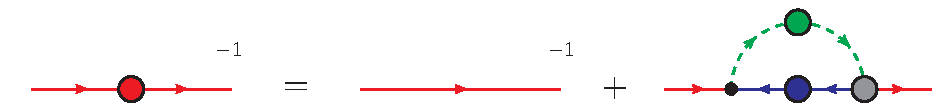
\includegraphics[width=0.8\textwidth]{figs/fermion_prop_DSE.pdf} \\
		\vspace{0.5cm}
		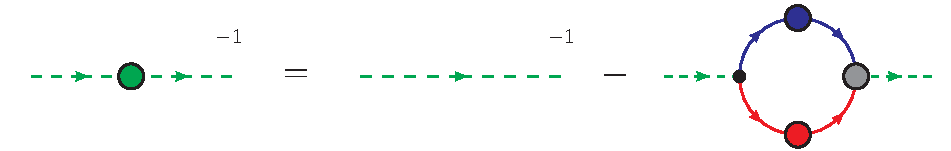
\includegraphics[width=0.8\textwidth]{figs/boson_prop_DSE.pdf} 
	\end{center}
	\caption[Coupled Dyson-Schwinger equations]{Coupled Dyson-Schwinger equations for the fermion and boson propagator. The red, blue and green blobs denote the full fermion and boson propagators. The black dot denotes the classical vertex $S^{(3)}$ and the gray blob denotes the full vertex $\Gamma^{(3)}$.}
	\label{fig:prop_DSEs}
\end{figure}

Inserting the classical propagators and the renormalized detuning from Eq.~\eqref{eq:renormalized-detuning} into the Dyson-Schwinger equations above yields the central equations of this work. Renaming the fermion propagator $G_{\psi} = G_{\psi\psi^*}$ and using $G^{-1}_{\psi} = \Gamma^{(2)}_{\psi\psi^*}$ and similarly for the boson gives
%
\begin{align}
	\label{eq:selfconsistent-equations}
	G^{-1}_{\psi}(\omega_n,\bm{p}) &= -i\omega_n+\bm{p}^2-\mu + \Sigma_{\psi}(\omega_n,\bm{p}) \,, \notag \\
	G^{-1}_{\phi}(\omega_n,\bm{p}) &= -\frac{h^2}{8\pi a} - \Pi_{\phi}(\omega_n,\bm{p}) \,,
\end{align}
%
where we defined the fermionic and bosonic self-energy, $\Sigma_{\psi}$ and $\Pi_{\phi}$, respectively. Using the classical Yukawa coupling $h$ for the vertices, the self-energies are given by
%
\begin{align}
	\label{eq:self-energies}
	\Sigma_{\psi}(\omega_n,\bm{p}) &= h^2 \int\frac{d^{3}q}{(2\pi)^{3}}\,T\sum_{\Omega_m} G_{\phi}(\Omega_m,\bm{q}) G_{\psi}(\Omega_m-\omega_n,\bm{q-p}) \,, \notag \\
	\Pi_{\phi}(\omega_n,\bm{p}) &= h^2 \int\frac{d^{3}q}{(2\pi)^{3}}\left[ T\sum_{\Omega_m} G_{\psi}(\Omega_m,\bm{q}) G_{\psi}(\omega_n-\Omega_m,\bm{p-q}) - \frac{1}{2\bm{q}^2} \right] \,,
\end{align}
%
where the last term was absorbed from the renormalized detuning to regularize the integral. Note that in the fermionic self-energy $\Sigma_{\psi}$, the sum is over bosonic Matsubara frequencies $\Omega_m=2m\pi T$, whereas in the bosonic self-energy $\Pi_{\phi}$, the sum is over fermionic Matsubara frequencies $\Omega_m=(2m+1)\pi T$.

Using the spectral representation in Eq.~\eqref{eq:spectral-representation} for the fermion and boson propagator, the self-energies can be written in terms of spectral loop integrals, 
%
\begin{align}
	\label{eq:spectral-self-energies}
	\Sigma_{\psi}(\omega_n,\bm{p}) &= h^2\int_{\bm{q},\lambda_1,\lambda_2}
	\rho_{\phi}(\lambda_1,\bm{q}) \rho_{\psi}(\lambda_2,\bm{q}-\bm{p})\,
	I_{\psi}(\omega_n,\lambda_1,\lambda_2) \,, \notag \\
	\Pi_{\phi}(\omega_n,\bm{p}) &= h^2\int_{\bm{q}} \left[\int_{\lambda_1,\lambda_2}
	\rho_{\psi}(\lambda_1,\bm{q}) \rho_{\psi}(\lambda_2,\bm{p}-\bm{q})\,
	I_{\phi}(\omega_n,\lambda_1,\lambda_2) - \frac{1}{2\bm{q}^2} \right] \,.
\end{align}
%
We use the notation $\int_{\bm{q}}=\int d^3q/(2\pi)^3$ and $\int_{\lambda}=\int_{-\infty}^{\infty}d\lambda$. The Matsubara summation in $I_{\psi}(\omega_n,\lambda_1,\lambda_2)$ and $I_{\phi}(\omega_n,\lambda_1,\lambda_2)$ can be carried out analytically, leaving us with symbolic expressions in terms of the argument $\omega_n$ for both self-energies, which can be evaluated at any complex frequency. The explicit calculation of the Matsubara sums can be found in Appendix~\ref{app:matsubara-sums} and a more detailed discussion in~\cite{Punk2010}.

The resulting expressions for $I_{\psi}(\omega_n,\lambda_1,\lambda_2)$ and $I_{\phi}(\omega_n,\lambda_1,\lambda_2)$ are given by
%
\begin{align}
	\label{eq:spectral-sums}
	I_{\psi}(\omega_n,\lambda_1,\lambda_2) &= T\sum_{\Omega_m} \frac{1}{i\Omega_m-\lambda_1}\frac{1}{i(\Omega_m-\omega_n)-\lambda_2} = \frac{-n_B(\lambda_1)-n_F(\lambda_2)}{-i\omega_n+\lambda_1-\lambda_2} \,, \notag \\
	I_{\phi}(\omega_n,\lambda_1,\lambda_2) &= T\sum_{\Omega_m} \frac{1}{i\Omega_m-\lambda_1}\frac{1}{i(\omega_n-\Omega_m)-\lambda_2} = \frac{1-n_F(\lambda_1)-n_F(\lambda_2)}{-i\omega_n+\lambda_1+\lambda_2} \,,
\end{align}
%
where $n_F(\lambda)=1/(e^{\lambda/T}+1)$ is the Fermi distribution function and $n_B(\lambda)=1/(e^{\lambda/T}-1)$ is the Bose-Einstein distribution function. For $T\rightarrow0$, the results simplify according to $n_B(\lambda)\rightarrow-\theta(-\lambda)$ and $n_F(\lambda)\rightarrow\theta(-\lambda)$, where $\theta(\lambda)$ is the Heaviside step function.

%%%%%%%%%%%%%%%%%%%%%%%%%%%%
\subsection*{Evaluation at real frequencies}
\label{sec:evaluation-real-frequencies}

The regularized and coupled DSEs in~\eqref{eq:selfconsistent-equations} can be evaluated at arbitrary complex frequencies. For the extraction of the spectral functions with~\eqref{eq:spectral-relation}, we choose $\omega_n=-i(\omega+i\varepsilon)$ with $\omega$ real and $\varepsilon\rightarrow 0^+$. The limit $\varepsilon\rightarrow 0^+$ is performed analytically using the relation
%
\begin{align}
	\label{eq:principal-value}
	\frac{1}{x\pm i0^+} = P\frac{1}{x} \mp i\pi\delta(x) \,,
\end{align}
%
where $P$ denotes the principal value. The delta function eliminates one spectral integration which allows us to write the imaginary part of the retarded self-energies as
%
\begin{align}
	\label{eq:imaginary-part-self-energies}
	\mathrm{Im}\,\Sigma^R_{\psi}(\omega,\bm{p}) &= \pi h^2\int_{\bm{q},\lambda}
	\rho_{\phi}(\omega+\lambda,\bm{q}) \rho_{\psi}(\lambda,\bm{q}-\bm{p})
	\left[-n_B(\omega+\lambda)-n_F(\lambda)\right] \,, \notag \\
	\mathrm{Im}\,\Pi^R_{\phi}(\omega,\bm{p}) &= \pi h^2\int_{\bm{q},\lambda}
	\rho_{\psi}(\omega-\lambda,\bm{q}) \rho_{\psi}(\lambda,\bm{p}-\bm{q})
	\left[1-n_F(\omega-\lambda)-n_F(\lambda)\right] \,.
\end{align}
%
Note that the pole of $n_B(\omega+\lambda)$ in the fermion self-energy is exactly canceled by the zero crossing of the boson spectral function $\rho_{\phi}$, see Section~\ref{section:spectral-representation}.

The real part of the retarded self-energies is obtained very efficiently from the imaginary part via the Kramers-Kronig relation~\cite{Abrikosov1975,Veillette2008},
%
\begin{align}
	\label{eq:kramers-kronig}
	\mathrm{Re}\,\Sigma^R(\omega,\bm{p}) = \frac{1}{\pi}\, P\int_{\lambda} \frac{\mathrm{Im}\, \Sigma^R(\lambda,\bm{p})}{\lambda-\omega} \,,
\end{align}
%
avoiding the 4-dimensional integrals in~\eqref{eq:spectral-self-energies} and performing a controlled 1-di\-men\-sio\-nal principal value integral instead. The fermionic self-energy decays for large values of the argument $\lambda$, see Appendix~\ref{app:fermion-self-energy-calculation}. Thus, the Kramers-Kronig relation can be used without further manipulations to compute the real part. As we will see later, the bosonic self-energy grows indefinitely for large values of $\lambda$ and requires special subtraction schemes to treat the divergent parts analytically. This has to do with the counterterm in~\eqref{eq:spectral-self-energies} and is discussed in detail in Appendix~\ref{app:boson-self-energy-calculation}.

Having obtained the real and imaginary part of the retarded self-energies, the spectral functions can be calculated with Eq.~\eqref{eq:spectral-relation}. More explicitly, for the fermions,
%
\begin{align}
	\label{eq:spectral-extraction}
	\rho_{\psi}(\omega,\bm{p}) = \frac{1}{\pi}\, \mathrm{Im}\, G^R_{\psi}(\omega,\bm{p}) = \frac{-\mathrm{Im}\,\Sigma^R_{\psi}(\omega,\bm{p})/\pi}{\left[\omega-\bm{p}^2+\mu-\mathrm{Re}\,\Sigma^R_{\psi}(\omega,\bm{p})\right]^2+\left[\mathrm{Im}\, \Sigma^R_{\psi}(\omega,\bm{p})\right]^2} \,.
\end{align}
%
This updated spectral function can be used in the next iteration to solve the coupled DSEs in Fig.~\ref{fig:prop_DSEs} selfconsistently until convergence is reached.


%%%%%%%%%%%%%%%%%%%%%%%%%%%%
\subsection*{First iteration of the boson self-energy}
\label{sec:first-iteration}

The iterative procedure is initialized with the first iteration of the boson self-energy, for which analytic results at finite and zero temperature can be derived. Inserting the classical fermion spectral function $\rho_{\psi}(\lambda,\bm{p})=\delta(\lambda-\bm{p}^2+\mu)$ in Eq.~\eqref{eq:spectral-self-energies} and performing the spectral integrals, we obtain the well-known expression for the non-selfconsistent retarded boson self-energy
%
\begin{align}
	\label{eq:non-selfconsistent-boson-self-energy}
	\Pi^R_{\phi}(\omega,\bm{p}) = h^2 \int_{\bm{q}}\left[ \frac{1-n_F(\varepsilon_{\bm{q}}-\mu) -n_F(\varepsilon_{\bm{p-q}}-\mu)}{-\omega+\varepsilon_{\bm{q}} + \varepsilon_{\bm{p-q}}-2\mu-i0^+} - \frac{1}{2\bm{q}^2}\right] \,,
\end{align}
%
where $\varepsilon_{\bm{p}}=\bm{p}^2$ is the classical momentum dispersion. At finite temperature, the imaginary part can be calculated analytically. The full calculation of the boson self-energy with general mass and spin-imbalance can be found in Appendix~\ref{app:boson-self-energy-calculation}. Here, we just state the result for the balanced case with equal mass and chemical potential.

For $y\geq 0$, the imaginary part at finite temperature is given by
%
\begin{align}
	\label{eq:boson-imaginary-part-finite-temp}
	\text{Im}\,\Pi^R_{\phi}(\omega,\bm{p}) = \frac{h^2}{8\pi} \left[ \sqrt{y} -
	\begin{cases}
		2\sqrt{y}\,n_F\left(y-\mu\right) & ,\, \bm{p}=\bm{0} \\
		\frac{T}{p} \ln\left( \frac{n_F(\mu-q_{+}^2)}{n_F(\mu-q_{-}^2)} \right) & ,\, \bm{p}\neq\bm{0}
	\end{cases} \right] \,,
\end{align}
%
where we have defined $y=\omega/2-p^2/4+\mu$ and $q_{\pm} = \sqrt{y}\pm p/2$, with $p=|\bm{p}|$. For $y<0$, the imaginary part vanishes identically. The real part at finite temperature cannot be solved analytically and has to be calculated numerically. However, at zero temperature, analytic expressions for both parts can be found. At $T=0$, the imaginary part is
%
\begin{align}
	\label{eq:boson-imaginary-part-zero-temp}
	\text{Im}\,\Pi^R_{\phi}(\omega,\bm{p}) = \frac{h^2}{8\pi} \left[ \sqrt{y} -
	\begin{cases}
		2\sqrt{y}\,\theta\left(\mu-y\right) & ,\, \bm{p}=\bm{0} \\
		\frac{\theta\left( \mu-
			q_{-}^2 \right)}{p} \left[
		\mu-q_{-}^2 -
		\left(\mu-q_{+}^2\right)
		\theta\left( \mu-q_{+}^2 \right)
		\right] & ,\, \bm{p}\neq\bm{0}
	\end{cases} \right] \,.
\end{align}
%
Note that the second term only contributes for $\mu>0$. The real part at vanishing spatial momentum, see Appendix~\ref{app:boson-self-energy-calculation}, is given for $\mu>0$ by
%
\begin{align}
	\label{eq:boson-real-part-zero-momentum}
	\text{Re}\, \Pi^R_{\phi}(\omega,\bm{0}) &= \frac{h^2}{2\pi^2} \left[ \sqrt{\mu} - \sqrt{|y|}
	\begin{cases}
		\text{arctanh}\left(\sqrt{\frac{\mu}{y}}\right) & ,\, y \geq 0 \\
		\arctan\left( \sqrt{\frac{\mu}{|y|}}\right)-\frac{\pi}{4} & ,\, y < 0
	\end{cases} \right]	\,.
\end{align}
%
For general non-zero spatial momentum, the expression is slightly more complicated
\begin{align}
	\label{eq:boson-real-part-general-momentum}
	\text{Re}\, \Pi^R_{\phi}(\omega,\bm{p}) =\,
	&\frac{h^2}{4\pi^2} \left[
	\sqrt{\mu} - \frac{y-\mu+p^2/4}{2p}\log\left(\frac{y-\tilde{q}^2_{+}}{y-\tilde{q}^2_{-}}\right)\right. \notag \\
	&- \sqrt{|y|}\left.
	\begin{cases}
		\text{arctanh}\left(\frac{\tilde{q}_{-}}{\sqrt{y}}\right) + 
		\text{arctanh}\left(\frac{\tilde{q}_{+}}{\sqrt{y}}\right) & ,\, y \geq 0 \\
		\text{arctan}\left(\frac{\tilde{q}_{-}}{\sqrt{|y|}}\right) +
		\text{arctan}\left(\frac{\tilde{q}_{+}}{\sqrt{|y|}}\right)-\frac{\pi}{2} & ,\, y < 0
	\end{cases}
	\right] \,,
\end{align}
with $\tilde{q}_{\pm} = \sqrt{\mu} \pm p/2$. For $\mu<0$, the real part is just given by $\text{Re}\, \Pi^R_{\phi}(\omega,\bm{p})=h^2\sqrt{-y}/(8\pi)$, where $y<0$. These results also agree with the formulas given in~\cite{Punk2010}.


\clearpage

\section{Superfluid phase}
\label{section:superfluid-phase}

In this Section, we consider the general case of a non-vanishing condensate expectation value ($\Delta\neq 0$). Now, we also have to account for the off-diagonal, also called anomalous, contributions. The general structure of the new DSEs is given by
%
\begin{align}
	\label{eq:matrix-DSE-structure}
	\begin{pmatrix}
		\Gamma^{(2)}_{11} & \Gamma^{(2)}_{12} \\
		\Gamma^{(2)}_{21} & \Gamma^{(2)}_{22}
	\end{pmatrix}
	=
	\begin{pmatrix}
		S^{(2)}_{11} & S^{(2)}_{12} \\
		S^{(2)}_{21} & S^{(2)}_{22}
	\end{pmatrix}
	-
	\begin{pmatrix}
		\Sigma_{11} & \Sigma_{12} \\
		\Sigma_{21} & \Sigma_{22}
	\end{pmatrix} \,,
\end{align}
%
and the components of the propagator are determined with Eq.~\eqref{eq:propagator-gamma} by a matrix inverse
%
\begin{align}
	\label{eq:matrix-propagator-inverse}
	\begin{pmatrix}
		G_{11} & G_{12} \\
		G_{21} & G_{22}
	\end{pmatrix}
	= \frac{1}{\Gamma^{(2)}_{11}\Gamma^{(2)}_{22}
		-\Gamma^{(2)}_{12}\Gamma^{(2)}_{21}}
	\begin{pmatrix}
		\Gamma^{(2)}_{22} & -\Gamma^{(2)}_{12} \\
		-\Gamma^{(2)}_{21} & \Gamma^{(2)}_{11}
	\end{pmatrix} \,.
\end{align}
%
This means that the fermion and boson propagators are now matrix objects with normal and anomalous components. For the balanced case, we choose the notation
%
\begin{align}
	\label{eq:matrix-propagators-components}
	G_{\Psi\Psi^{\dagger}} =
	\begin{pmatrix}
		G_{\uparrow\uparrow} & G_{\uparrow\downarrow} \\
		G_{\downarrow\uparrow} & G_{\downarrow\downarrow}
	\end{pmatrix} \,, \qquad
	G_{\Phi\Phi^{\dagger}} =
	\begin{pmatrix}
		G_{\phi\phi^*} & G_{\phi\phi} \\
		G_{\phi^*\phi^*} & G_{\phi^*\phi}
	\end{pmatrix} \,.
\end{align}
%
Owing to the symmetry identities introduced in Section~\ref{section:nambu-gorkov-formalism}, the only independent components for the balanced Fermi gas are $G_{\uparrow\uparrow}$, $G_{\uparrow\downarrow}$, $G_{\phi\phi^*}$ and $G_{\phi\phi}$. Thus, each propagator is described completely by one normal and one anomalous component. Consequently, we now have four, instead of two, coupled equations, i.e., the normal components also depend on the anomalous components. For more details, also on the more general spin-imbalanced case, see~\cite{Frank2018}. The additional DSEs for the anomalous components can be derived by the same means from the master DSE in Eq.~\eqref{eq:DSE-general}, see Appendix~\ref{app:derivation-dse}. Using the new notation, the fermion DSEs in the symmetry-broken phase are given by\footnote{Note the different sign as compared to~\cite{Haussmann2009} for the anomalous component, see also~\cite{Andrenacci2003,Frank2018,Pieri2004-1}.}
%
\begin{align}
	\label{eq:fermion-DSEs-general}
	\Gamma^{(2)}_{\uparrow\uparrow}(P) &= S^{(2)}_{\uparrow\uparrow}(P) + h^2 \int_Q G_{\phi\phi^*}(Q) \cdot G_{\uparrow\uparrow}(Q-P)  \,, \notag \\
	\Gamma^{(2)}_{\uparrow\downarrow}(P) &= S^{(2)}_{\uparrow\downarrow}(P) - h^2 \int_Q G_{\phi\phi}(Q) \cdot G_{\uparrow\downarrow}(Q-P) \,,
\end{align}
%
where $P=(\omega_n,\bm{p})$ and $\int_Q=T\sum_{\Omega_n}\int_{\bm{q}}$. Analogously, the boson DSEs are given by
%
\begin{align}
	\label{eq:boson-DSEs-general}
	\Gamma^{(2)}_{\phi\phi^*}(P) &= S^{(2)}_{\phi\phi^*}(P) - h^2 \int_Q G_{\uparrow\uparrow}(Q) \cdot G_{\uparrow\uparrow}(P-Q) \,, \notag \\
	\Gamma^{(2)}_{\phi\phi}(P) &= S^{(2)}_{\phi\phi}(P) + h^2 \int_Q G_{\uparrow\downarrow}(Q) \cdot G_{\uparrow\downarrow}(P-Q) \,.
\end{align}
%
The classical inverse fermion and boson Green's functions are given by
%
\begin{align}
	\label{eq:classical-propagators-components}
	S^{(2)}_{\Psi\Psi^{\dagger}} =
	\begin{pmatrix}
		-i\omega_n+\xi_{\bm{p}} & \Delta \\
		\Delta & -i\omega_n-\xi_{\bm{p}}
	\end{pmatrix} \,, \qquad
	S^{(2)}_{\Phi\Phi^{\dagger}} =
	\begin{pmatrix}
		\nu & 0 \\
		0 & \nu
	\end{pmatrix} \,.
\end{align}
%
For more details on the symmetries between the components and the evaluation at real frequencies, see Appendix~\ref{app:derivation-dse} and~\cite{Pieri2004-1}.


%%%%%%%%%%%%%%%%%%%%%%%%%%%%
\section{Results}
\label{section:results}

In this Section, we discuss the numerical results obtained in this work. In the first part, we focus on the novel results for the non-perturbative spectral functions calculated directly in real frequencies and compare with other approaches. In the following parts, we benchmark our method against existing results for the unitary Fermi gas and compare with experimental data from MIT~\cite{Mukherjee2019}.


\subsection*{Spectral functions}
\label{subsection:spectral-functions}

We start with a discussion of the results for the spin-balanced Fermi gas in the normal phase. For details on the numerical implementation, we refer the reader to Appendix~\ref{app:numerical-implementation}.

Physical properties and reconstructions of the fermion spectral function have been discussed extensively in the literature~\cite{Haussmann2009,Palestini2012,Reichl2015}. However, fully selfconsistent results obtained directly in real-time are limited. Simultaneously with the spectral approach developed in this work, there have been other unpublished works by Johannes Lang and Tilman Enss based on the Keldysh formalism. In particular, the code of Johannes Lang is based on a fast Fourier transform to real-times that renders the convolutions in the self-energy expressions to simple matrix multiplications~\cite{Lang2023}. It was originally developed for general dynamic systems out of equilibrium and will be used to compare with our results in thermal equilibrium. In this part, we also show the bosonic dimer spectral function which has not received much attention in the past.

\begin{figure*}[b]
	\centering
	\subfigure[$(k_Fa)^{-1}=-0.5$]{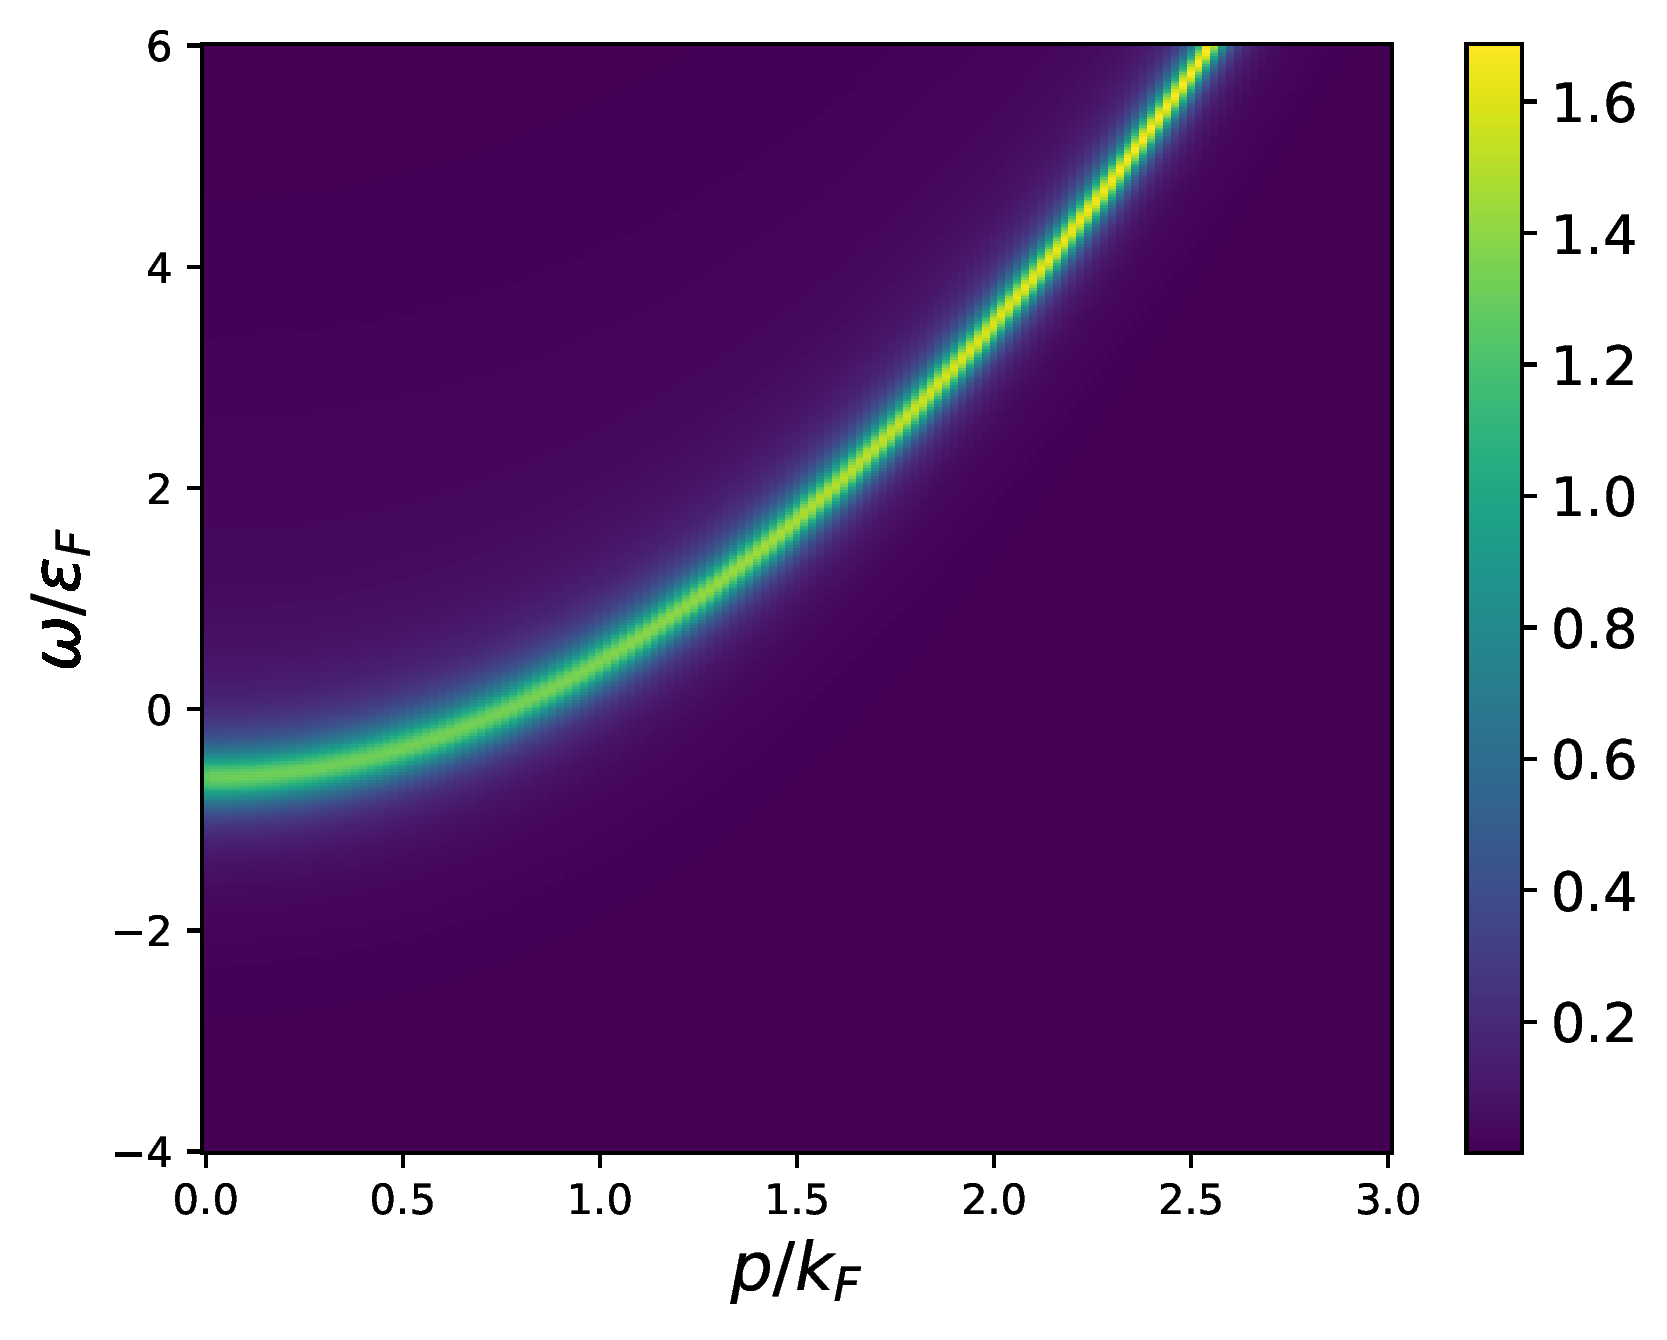
\includegraphics[width=0.32\textwidth]{figs/ferm_spec_kFa=-0.5.png}}
	\subfigure[$(k_Fa)^{-1}=0$]{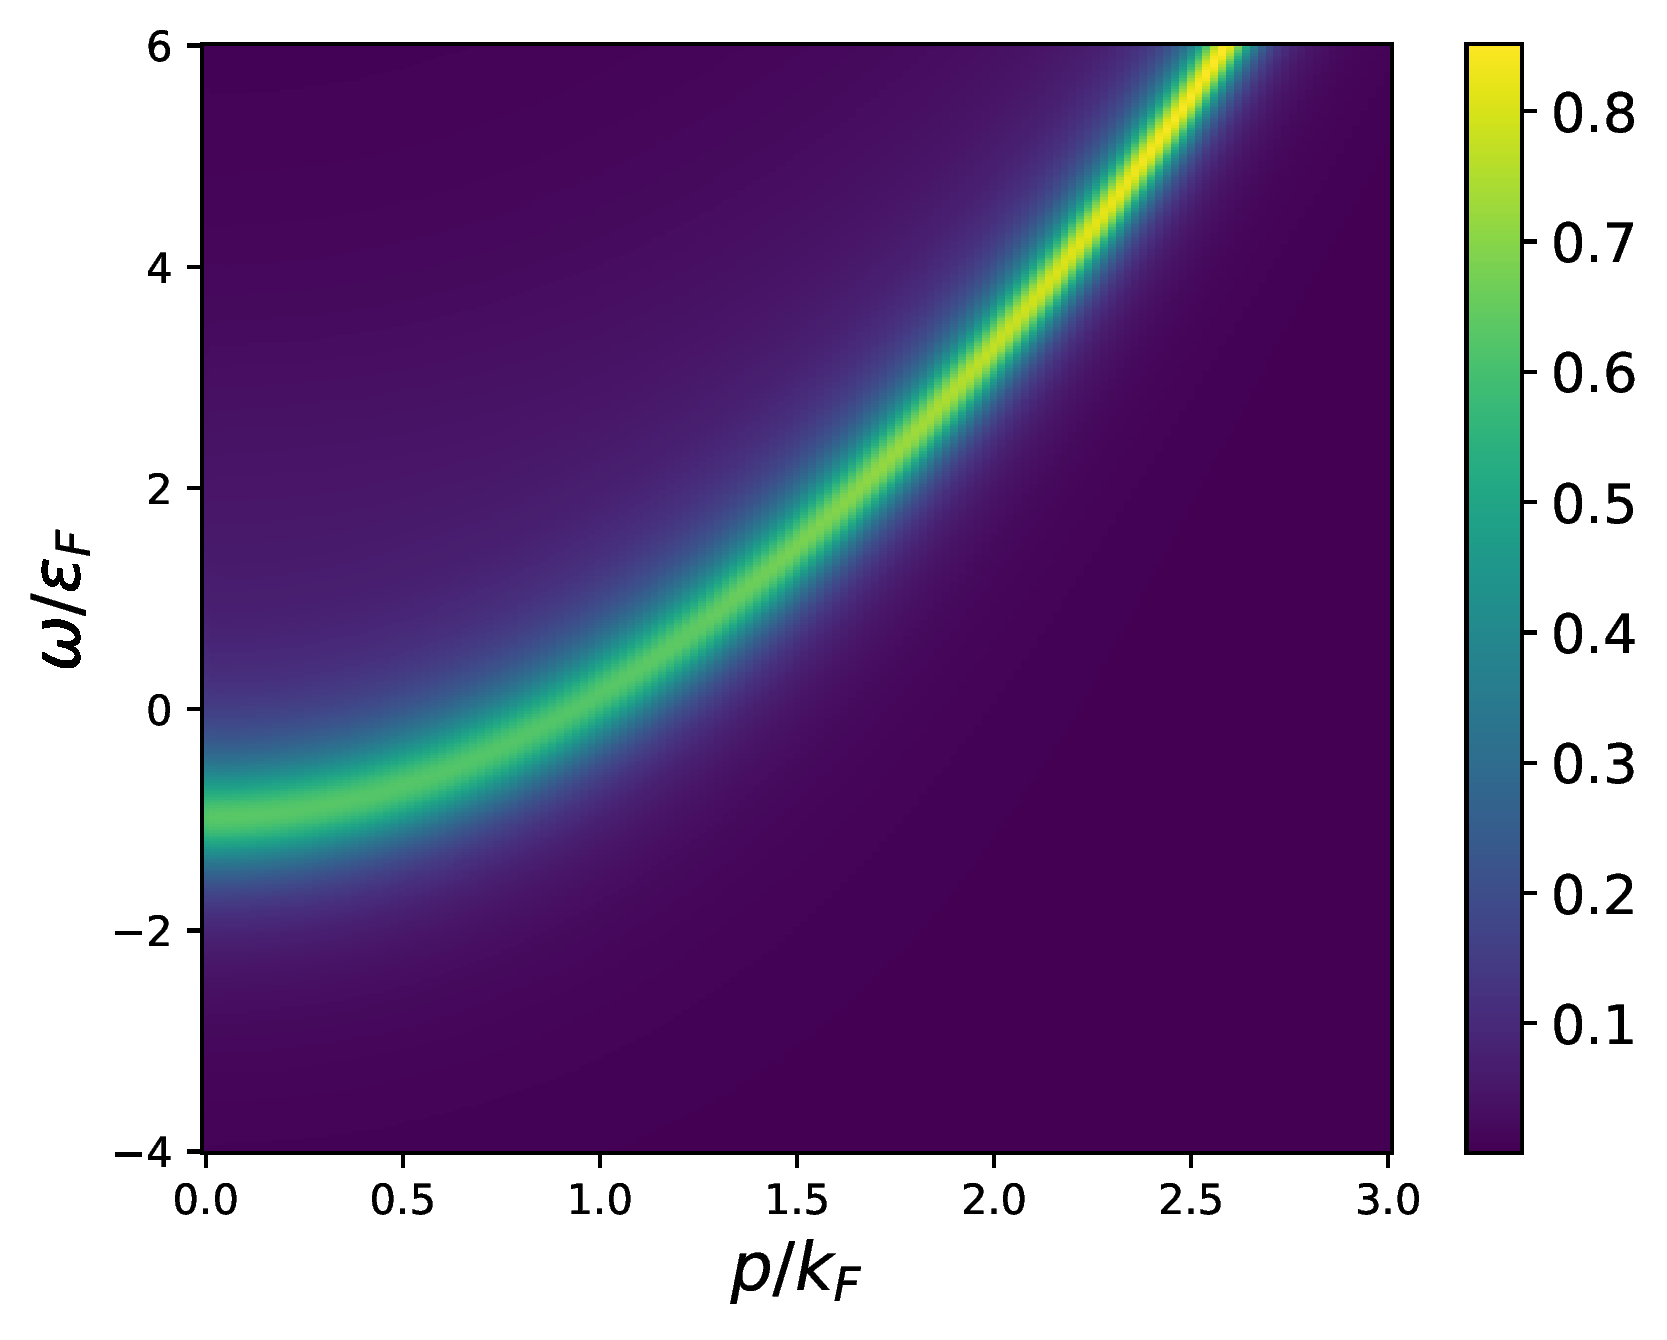
\includegraphics[width=0.32\textwidth]{figs/ferm_spec_kFa=0.png}}
	\subfigure[$(k_Fa)^{-1}=0.5$]{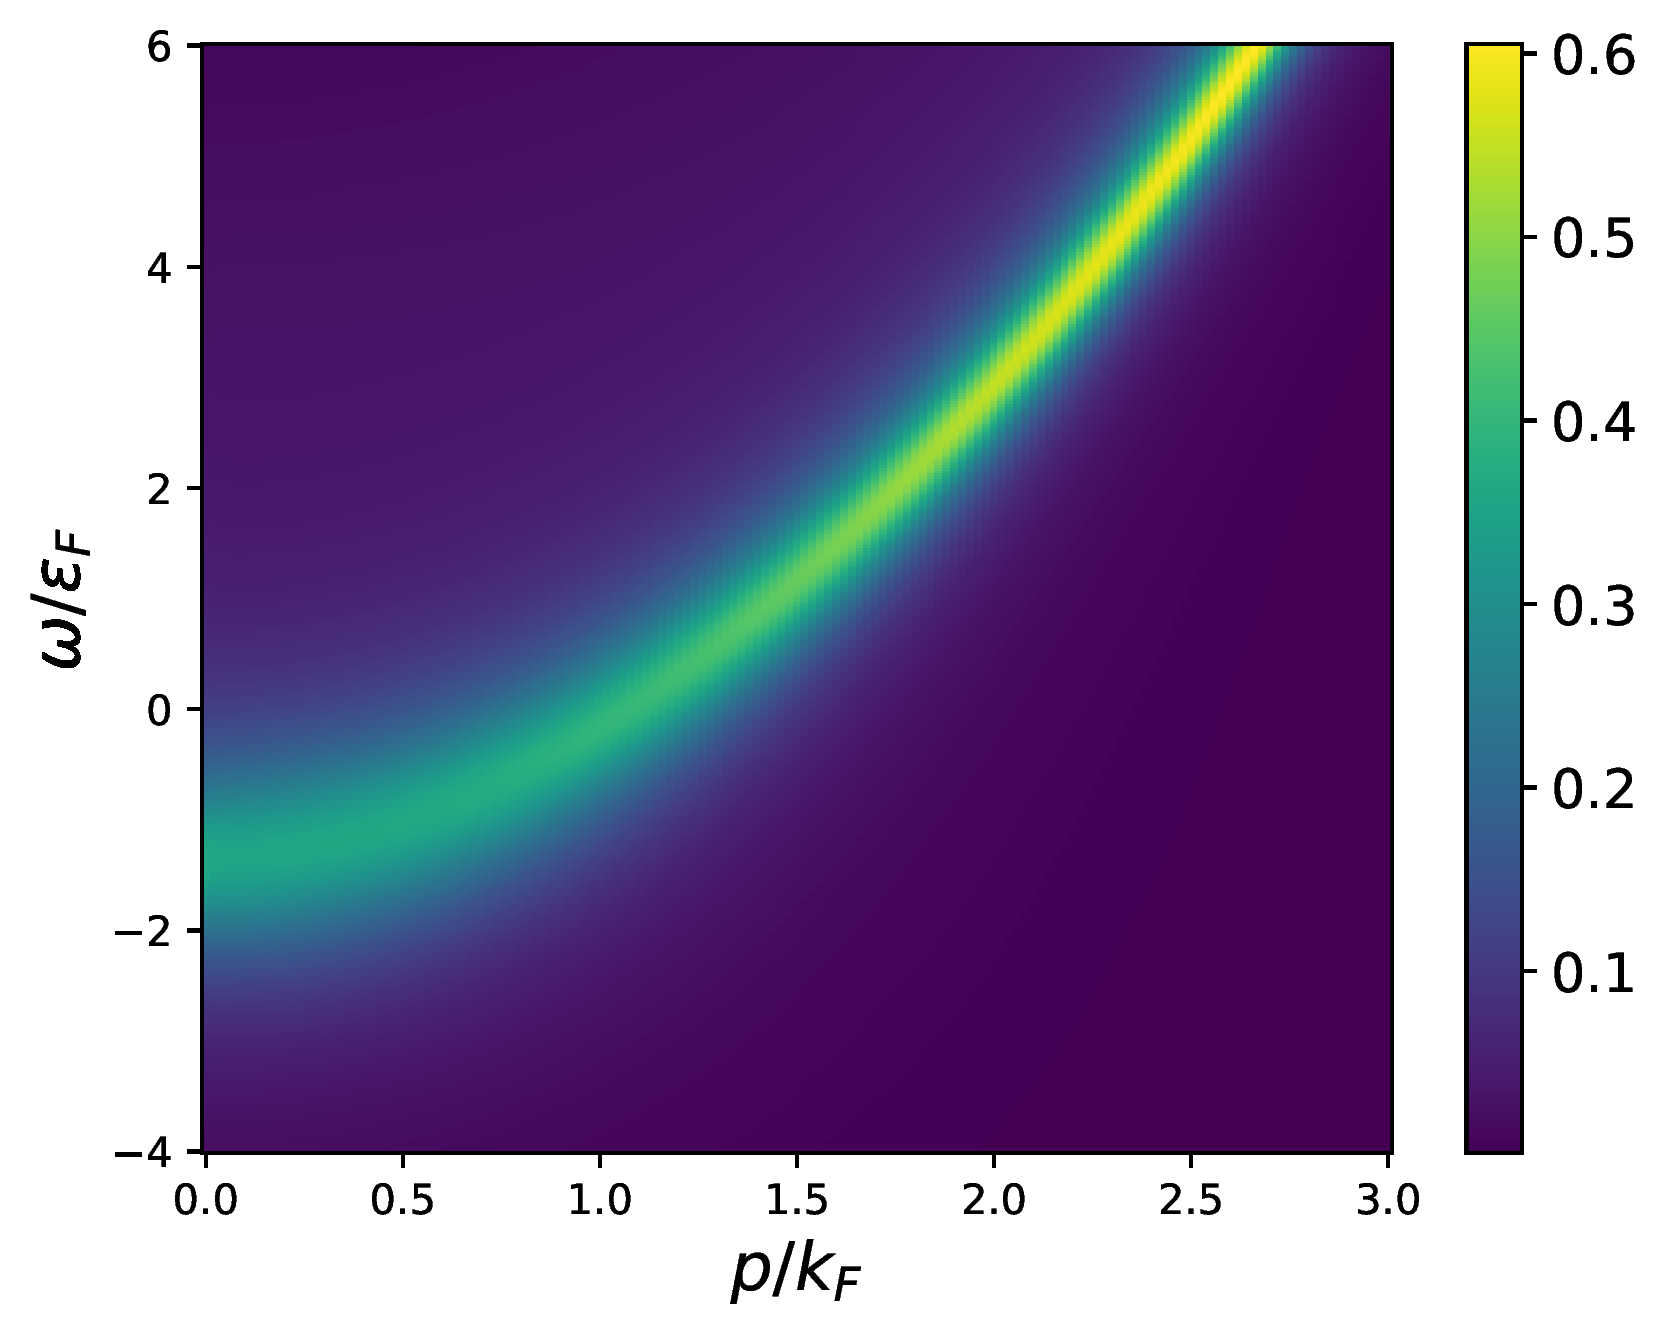
\includegraphics[width=0.32\textwidth]{figs/ferm_spec_kFa=0.5.png}}
	\caption[Fermion spectral function $\rho_{\psi}$ at different interaction strengths]{Results for the normalized fermionic spectral function $\rho_{\psi}\,\varepsilon_F$ for $\beta\mu=0.13146$ at different interaction strengths $(k_Fa)^{-1}$ which correspond to (a) BCS regime (b) unitarity (c) BEC regime.}
	\label{fig:fermion-specs}
\end{figure*}
%
\begin{figure*}[h]
	\centering
	\subfigure[$(k_Fa)^{-1}=-0.5$]{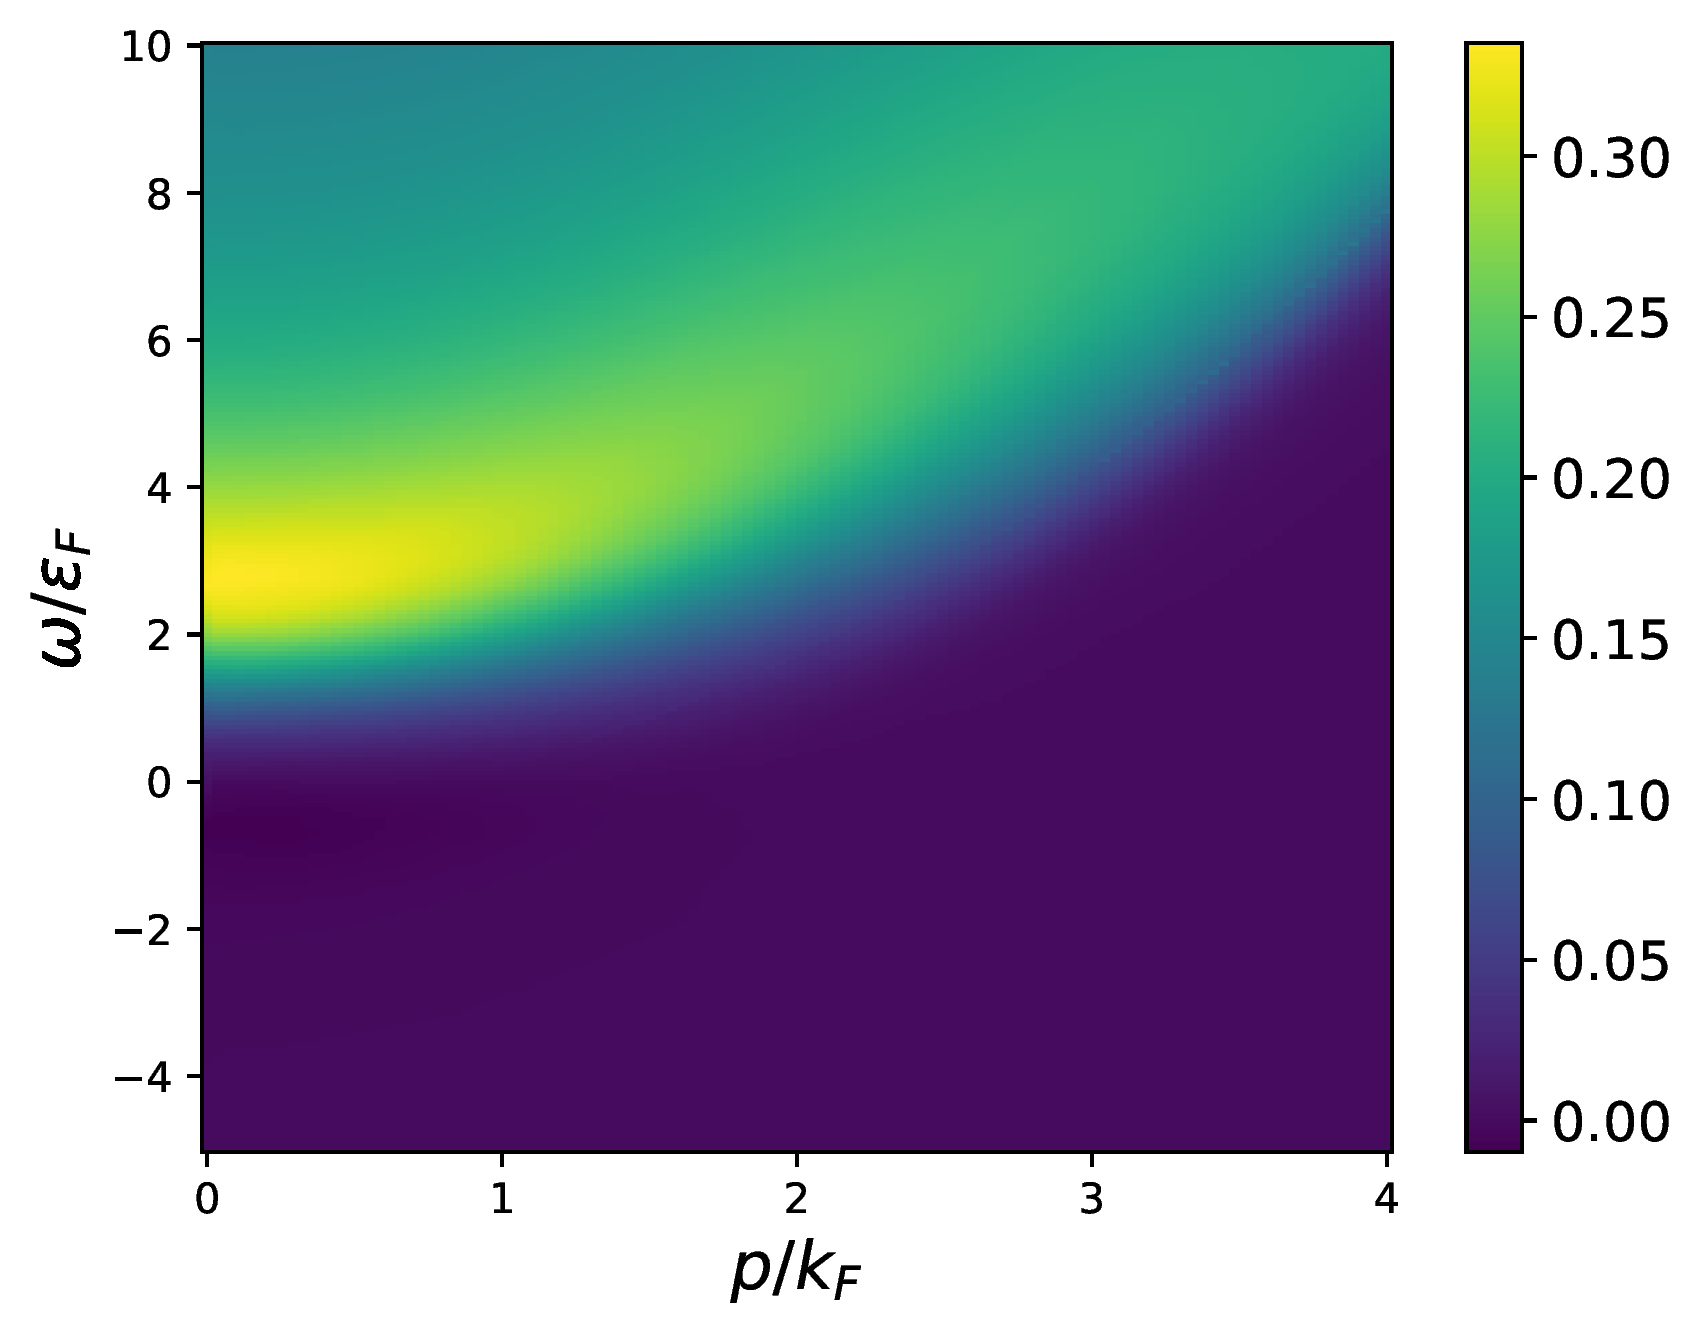
\includegraphics[width=0.328\textwidth]{figs/bos_spec_kFa=-0.5.png}}
	\subfigure[$(k_Fa)^{-1}=0$]{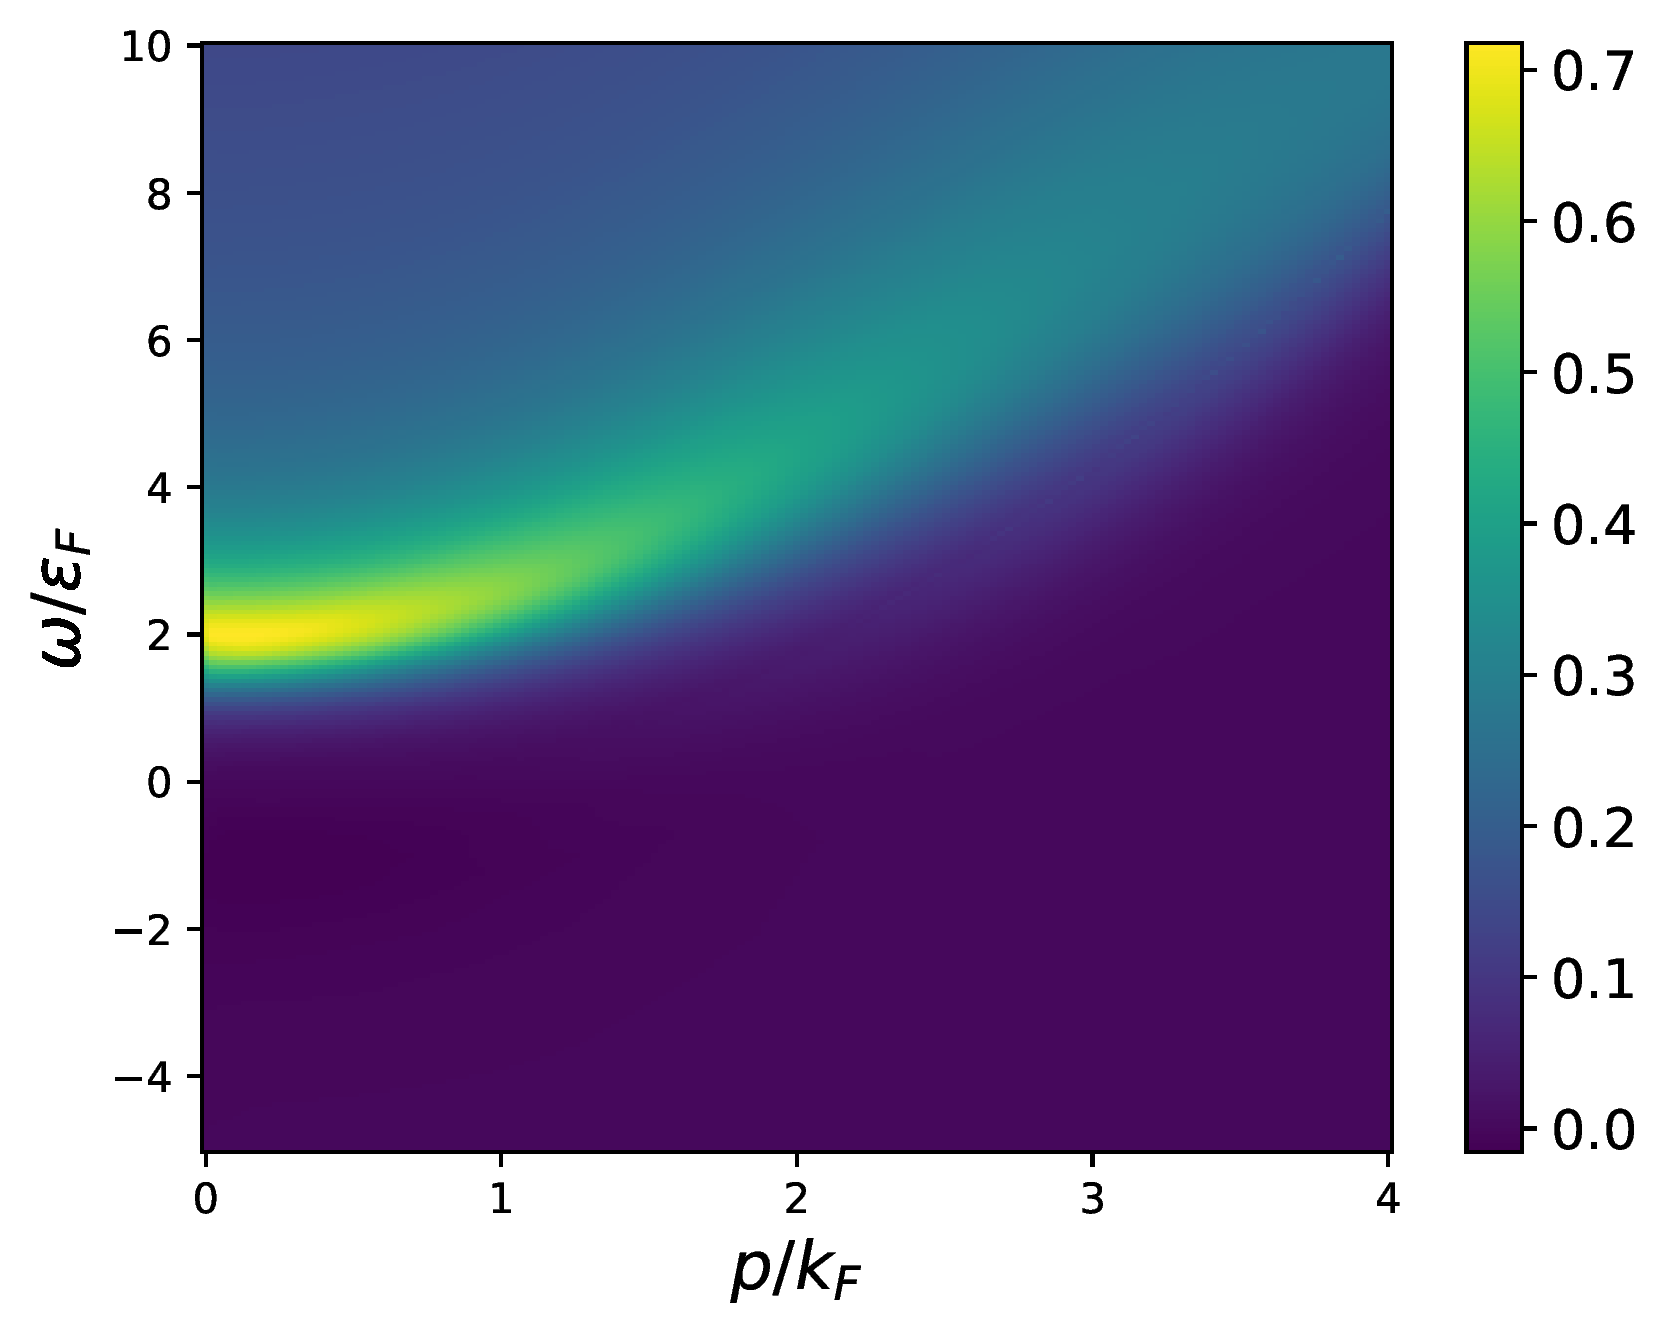
\includegraphics[width=0.32\textwidth]{figs/bos_spec_kFa=0.png}}
	\subfigure[$(k_Fa)^{-1}=0.5$]{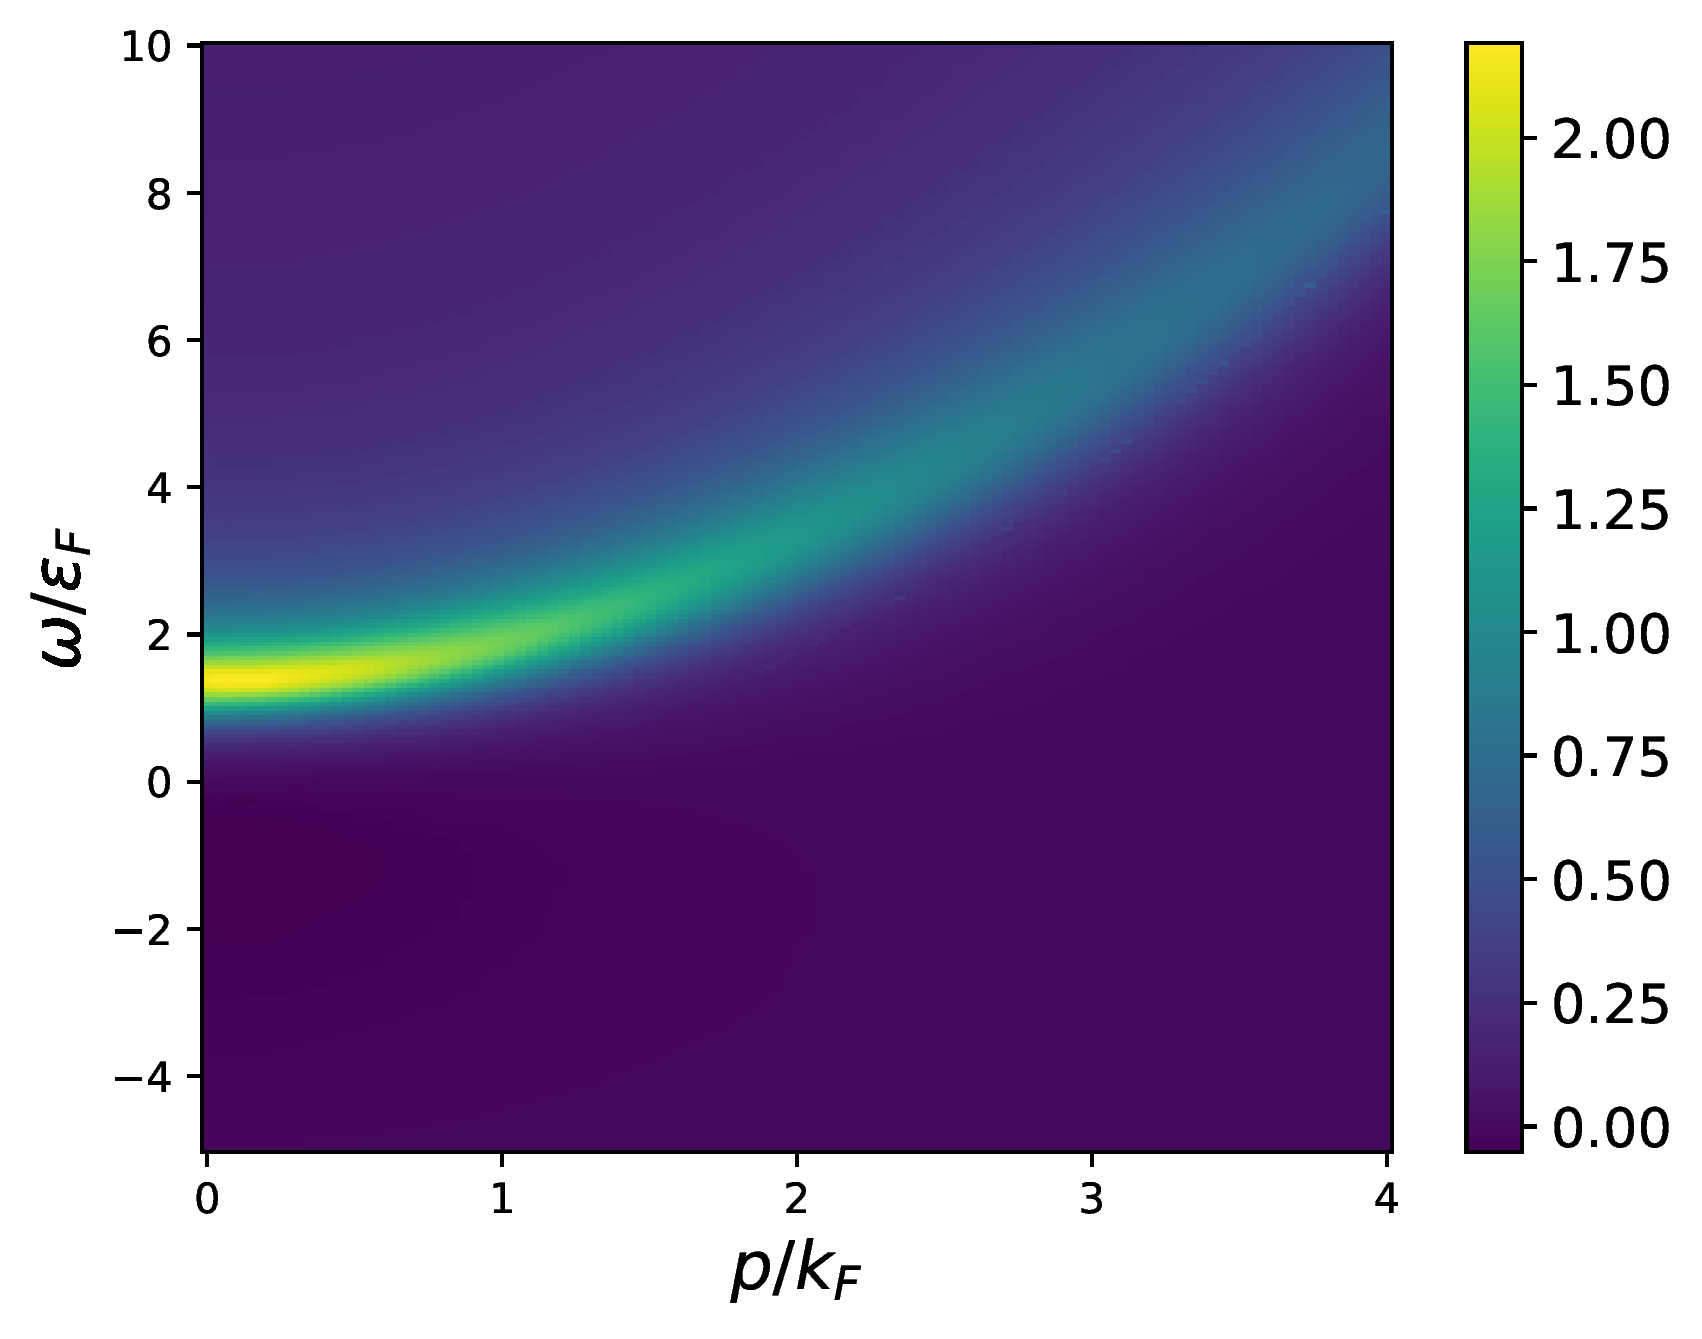
\includegraphics[width=0.328\textwidth]{figs/bos_spec_kFa=0.5.png}}
	\caption[Boson spectral function $\rho_{\phi}$ at different interaction strengths]{Results for the normalized bosonic dimer spectral function $h^2\rho_{\phi}\,\varepsilon_F/(8\pi)$ for $\beta\mu=0.13146$ at different interaction strengths $(k_Fa)^{-1}$ which correspond to (a) BCS regime (b) unitarity (c) BEC regime.}
	\label{fig:boson-specs}
\end{figure*}

Let us begin with the final results for the full momentum-dependent spectral functions at different interaction strengths. Fig.~\ref{fig:fermion-specs} shows results for the fermion spectral function $\rho_{\psi}$ and Fig.~\ref{fig:boson-specs} shows the corresponding bosonic dimer spectral functions $\rho_{\phi}$. In our unit system introduced in Chapter~\ref{chapter:introduction}, the frequency $\omega$ and momentum $p$ are measured in $\varepsilon_F$ and $k_F$, respectively, and the spectral functions have units of $\varepsilon^{-1}_F$. We state all results in dimensionless form. Note that the bosonic dimer spectral function is not normalized and depends on the choice of the Feshbach coupling $h$. In this way, it can be regarded as a pure interaction exchange boson and not a real particle. To eliminate the $h$-dependence, we multiply $\rho_{\phi}$ by $h^2/(8\pi)$ since $h^2G_{\phi}/(8\pi)$ is the relevant quantity which is related to the scattering amplitude, see Appendix~\ref{app:renormalization}.

The results for the bosonic dimer spectral function encode important information about the physics of the ultracold Fermi gas. First, we see a very broad peak structure for attractive interactions in the BCS regime, and a very sharp peak structure for repulsive interactions in BEC regime. This refers to the physical interpretation of condensed bosons on the BEC side. On this side of the BCS-BEC phase diagram, at $1/(k_Fa)=0.5$, the boson spectral function is very sharp and the system can be described as normal Bose liquid. On the BCS side of the crossover, at $1/(k_Fa)=-0.5$, the fermion spectral function is sharper and the system is described by a normal Fermi liquid, see Fig.~\ref{fig:crossover-phase-diagram}.

Fig.~\ref{fig:spec-convergence} shows the convergence behavior of the fermionic spectral function at unitarity for different temperatures. One can see that the spectral function at higher temperature convergences much faster than the spectral function at lower temperature. At $T=1.0\,T_F$, convergence is reached already after 6-7 iterations while the spectral function at $T=0.3\,T_F$ still varies considerably. Note the slow alternating convergence of the peak. This has to do with the fact that the bosonic spectral function gets very sharp and sensitive at lower temperatures close to the critical point, which will be discussed later in this Section. Without special treatment, like fixing the position of the boson peak or updating the spectral functions only partially~\cite{Frank2018}, it takes around 20 iterations to fully converge at $T=0.3\,T_F$. 

The fully converged fermion spectral functions obtained in this work are compared to the Keldysh results of Johannes Lang~\cite{Lang2023} in Fig.~\ref{fig:spec-comparison}. We find remarkable agreement between the two real-time approaches. However, a small residual shift of the peak positions is noticeable, which may result from remaining numerical issues. Nevertheless, a reconstruction from imaginary-time calculations by J. Lang via the Maximum Entropy Method~\cite{Jarrell2012} shows that the resulting spectral functions depend highly on the primer and may vary significantly. Without any prior information, the reconstructions differ notably from the real-time results. On the contrary, with real-time spectral functions as primer, the reconstructions yield the same results confirming the real-time calculations~\cite{Lang2023}. This shows the importance of computations directly in real frequencies.


\begin{figure}[h]
	\centering
	\subfigure[$T=0.3\,T_F$]{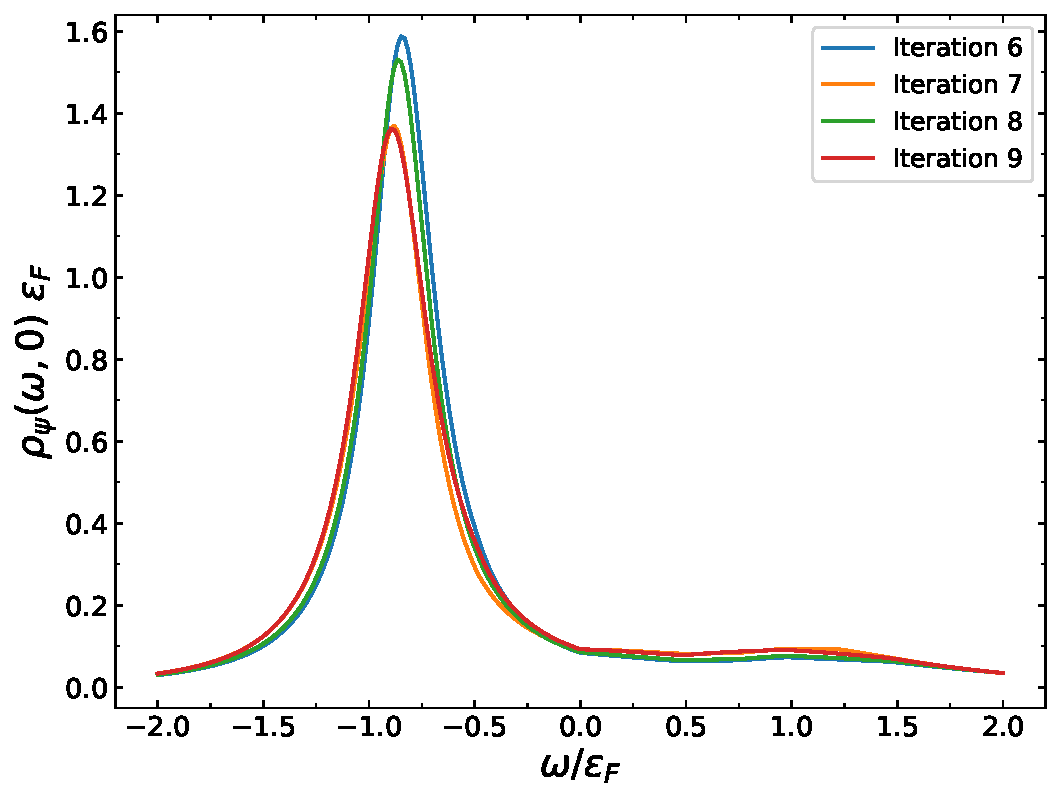
\includegraphics[width=0.47\textwidth]{figs/T=0.3_convergence.pdf}}
	\subfigure[$T=1.0\,T_F$]{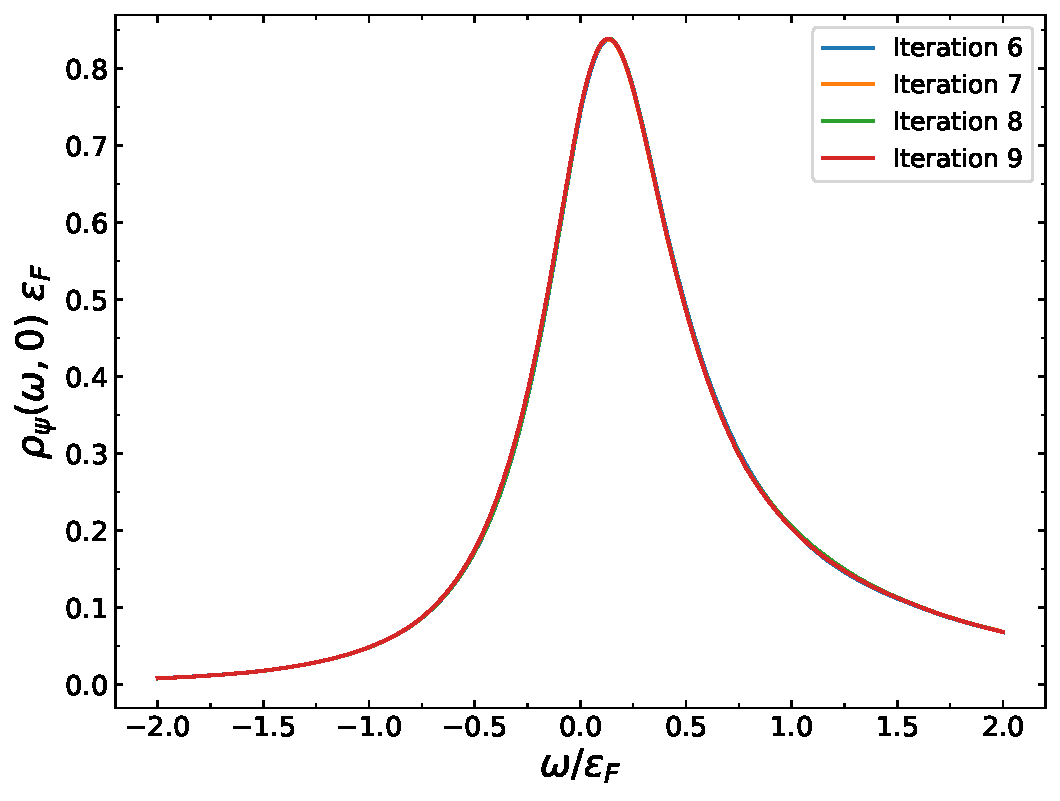
\includegraphics[width=0.47\textwidth]{figs/T=1_convergence.pdf}}
	\caption[Convergence of fermion spectral function at different temperatures]{Convergence of the fermionic spectral function at different temperatures.}
	\label{fig:spec-convergence}
\end{figure}


\begin{figure}[h]
	\centering
	\subfigure[$T=0.3\,T_F$]{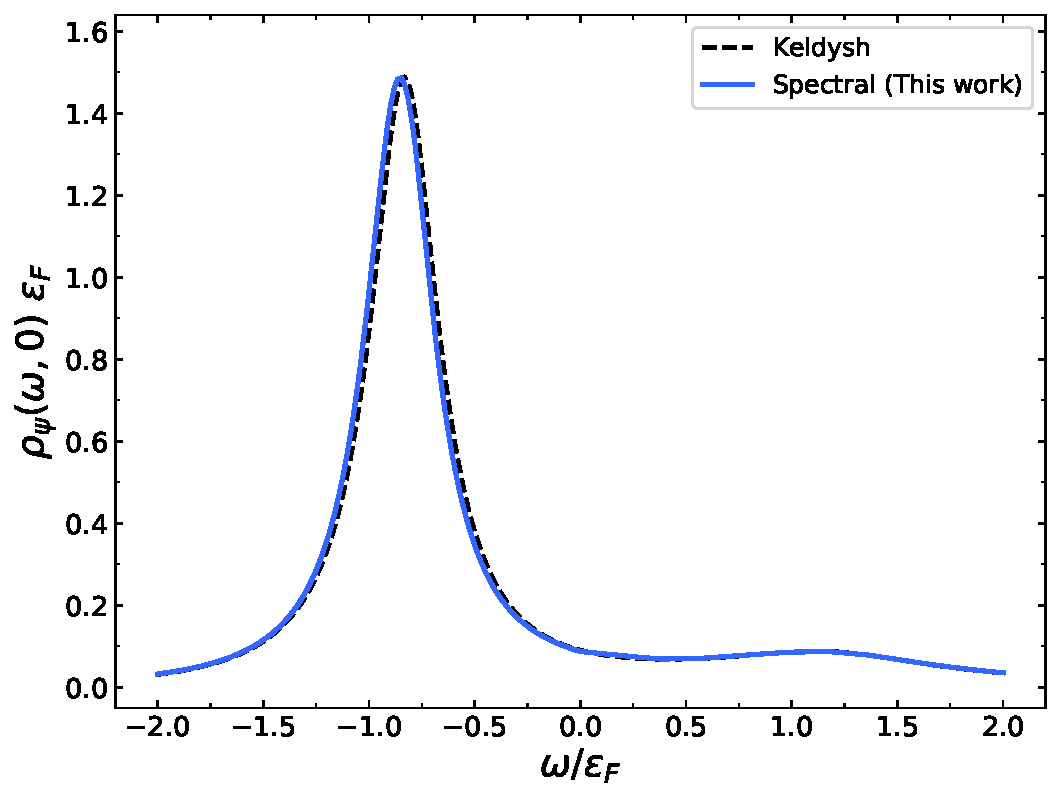
\includegraphics[width=0.47\textwidth]{figs/keldysh_comparison_T=0.3.pdf}}
	\subfigure[$T=1.0\,T_F$]{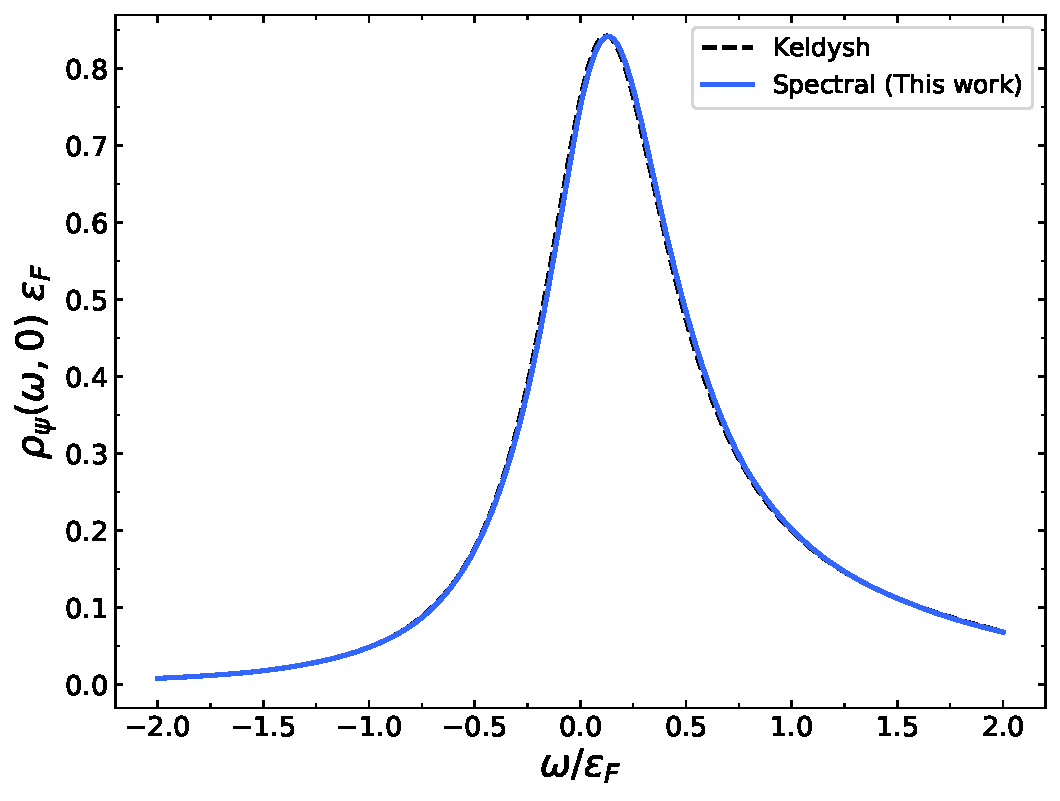
\includegraphics[width=0.47\textwidth]{figs/keldysh_comparison_T=1.pdf}}
	\caption[Comparison of spectral functions with the Keldysh approach]{Comparison of the fully converged fermionic spectral functions with a different real-time approach~\cite{Lang2023}, see explanations in the main text.}
	\label{fig:spec-comparison}
\end{figure}


Close to the critical temperature, the convergence behavior gets very problematic. Fig.~\ref{fig:fermion-specs-critical} and~\ref{fig:boson-specs-critical} show the fermion and boson spectral function for two consecutive iterations at $\beta\mu=2$. Similar to the oscillations in Fig.~\ref{fig:spec-convergence} at $T=0.3\,T_F$, we see the spectral functions alternating between two shapes, however, much more extreme. This situation can become very unstable and even increase in amplitude such that convergence is never reached. The reason for this is that the peak of the bosonic spectral function gets very sharp and sensitive at $\omega=0$ close to the critical temperature. Small numerical uncertainties in the fermion spectral function can lead to shifts of the bosonic peak below $\omega=0$, as can be seen in Fig.~\ref{fig:boson-specs-critical}. However, this situation is unphysical and numerically unstable, and leads to precondensed fermion spectral functions, see Fig.~\ref{fig:fermion-specs-critical}. In these cases, it is advisable to fix the boson peak at a certain value and then convert to the right interaction strength after convergence~\cite{Lang2023}. Another approach is to update the fermion spectral functions only partially to improve the convergence behavior~\cite{Frank2018}.

\begin{figure*}[t]
	\centering
	\subfigure[Iteration 7]{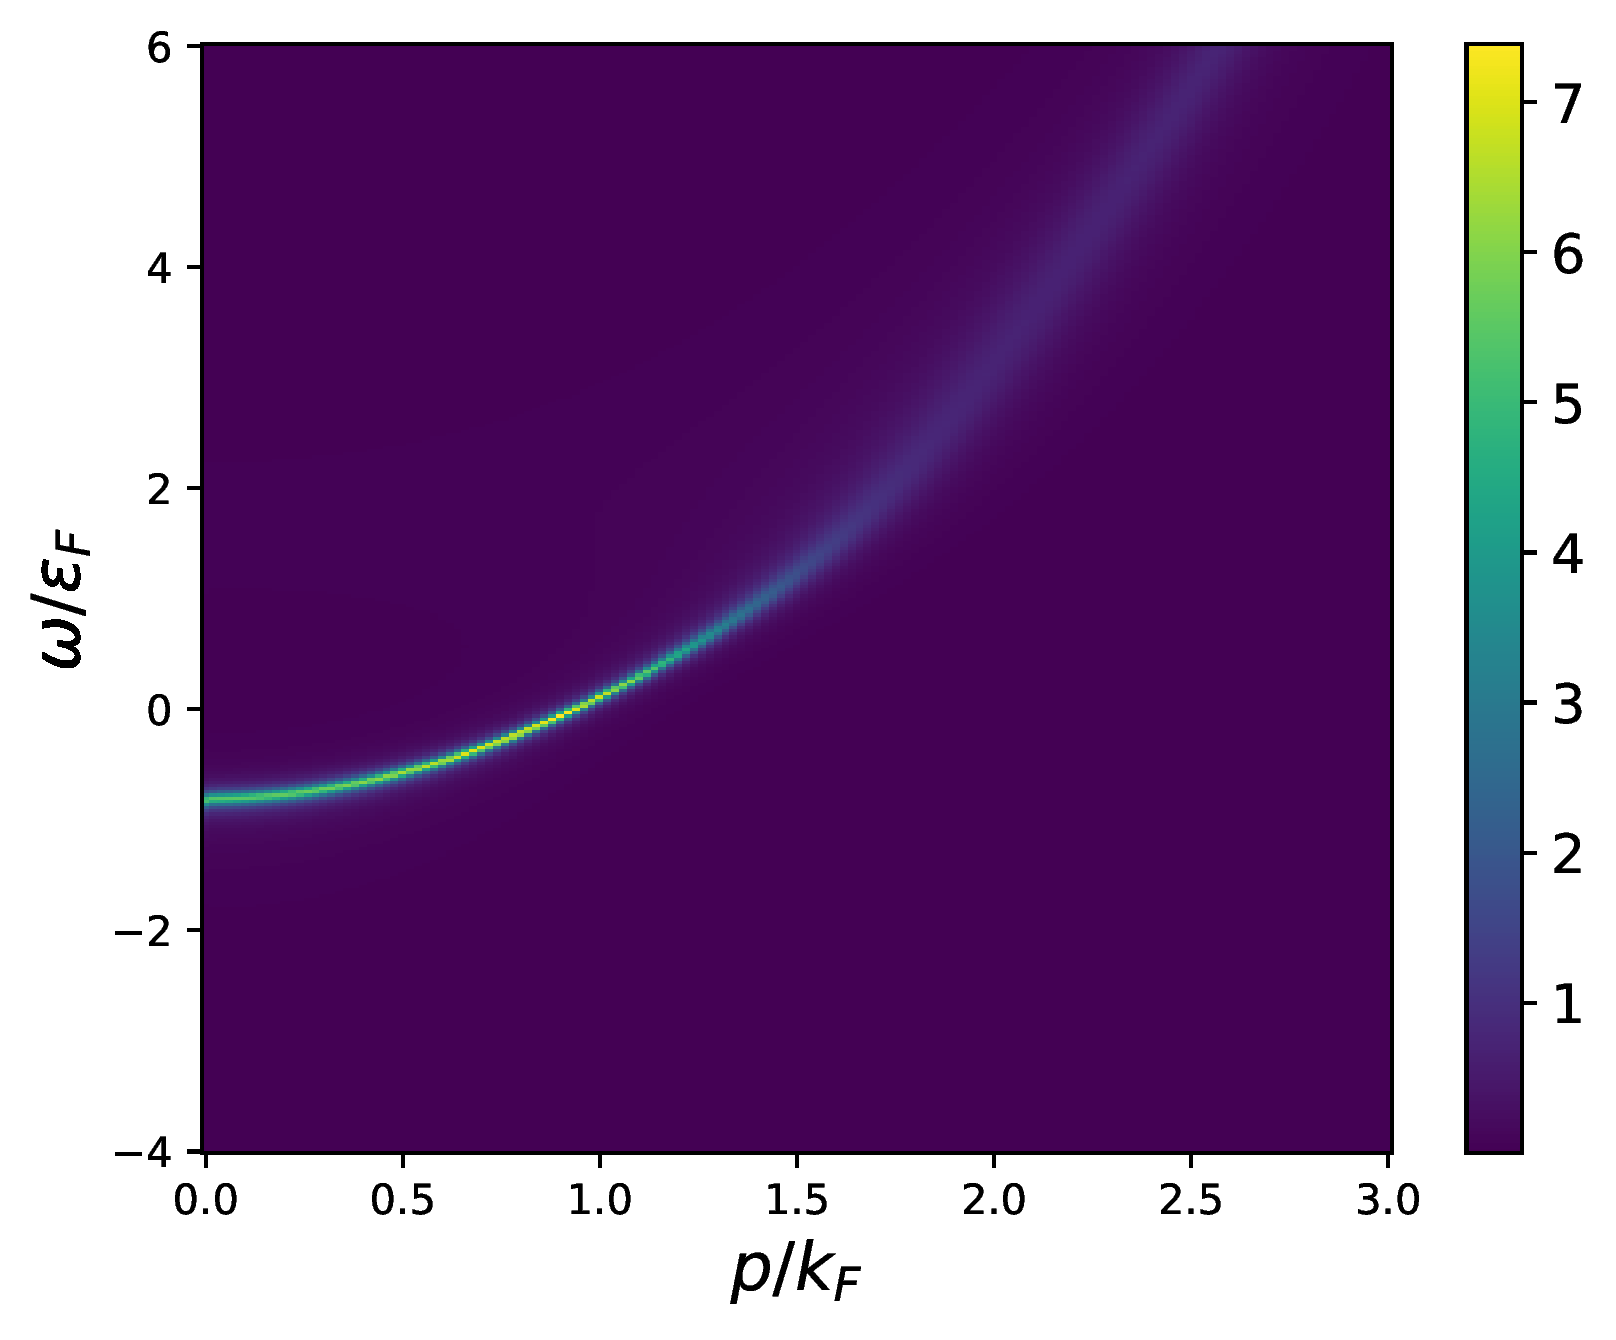
\includegraphics[width=0.39\textwidth]{figs/fermion_T=0.2_iter=7.png}}
	\subfigure[Iteration 8]{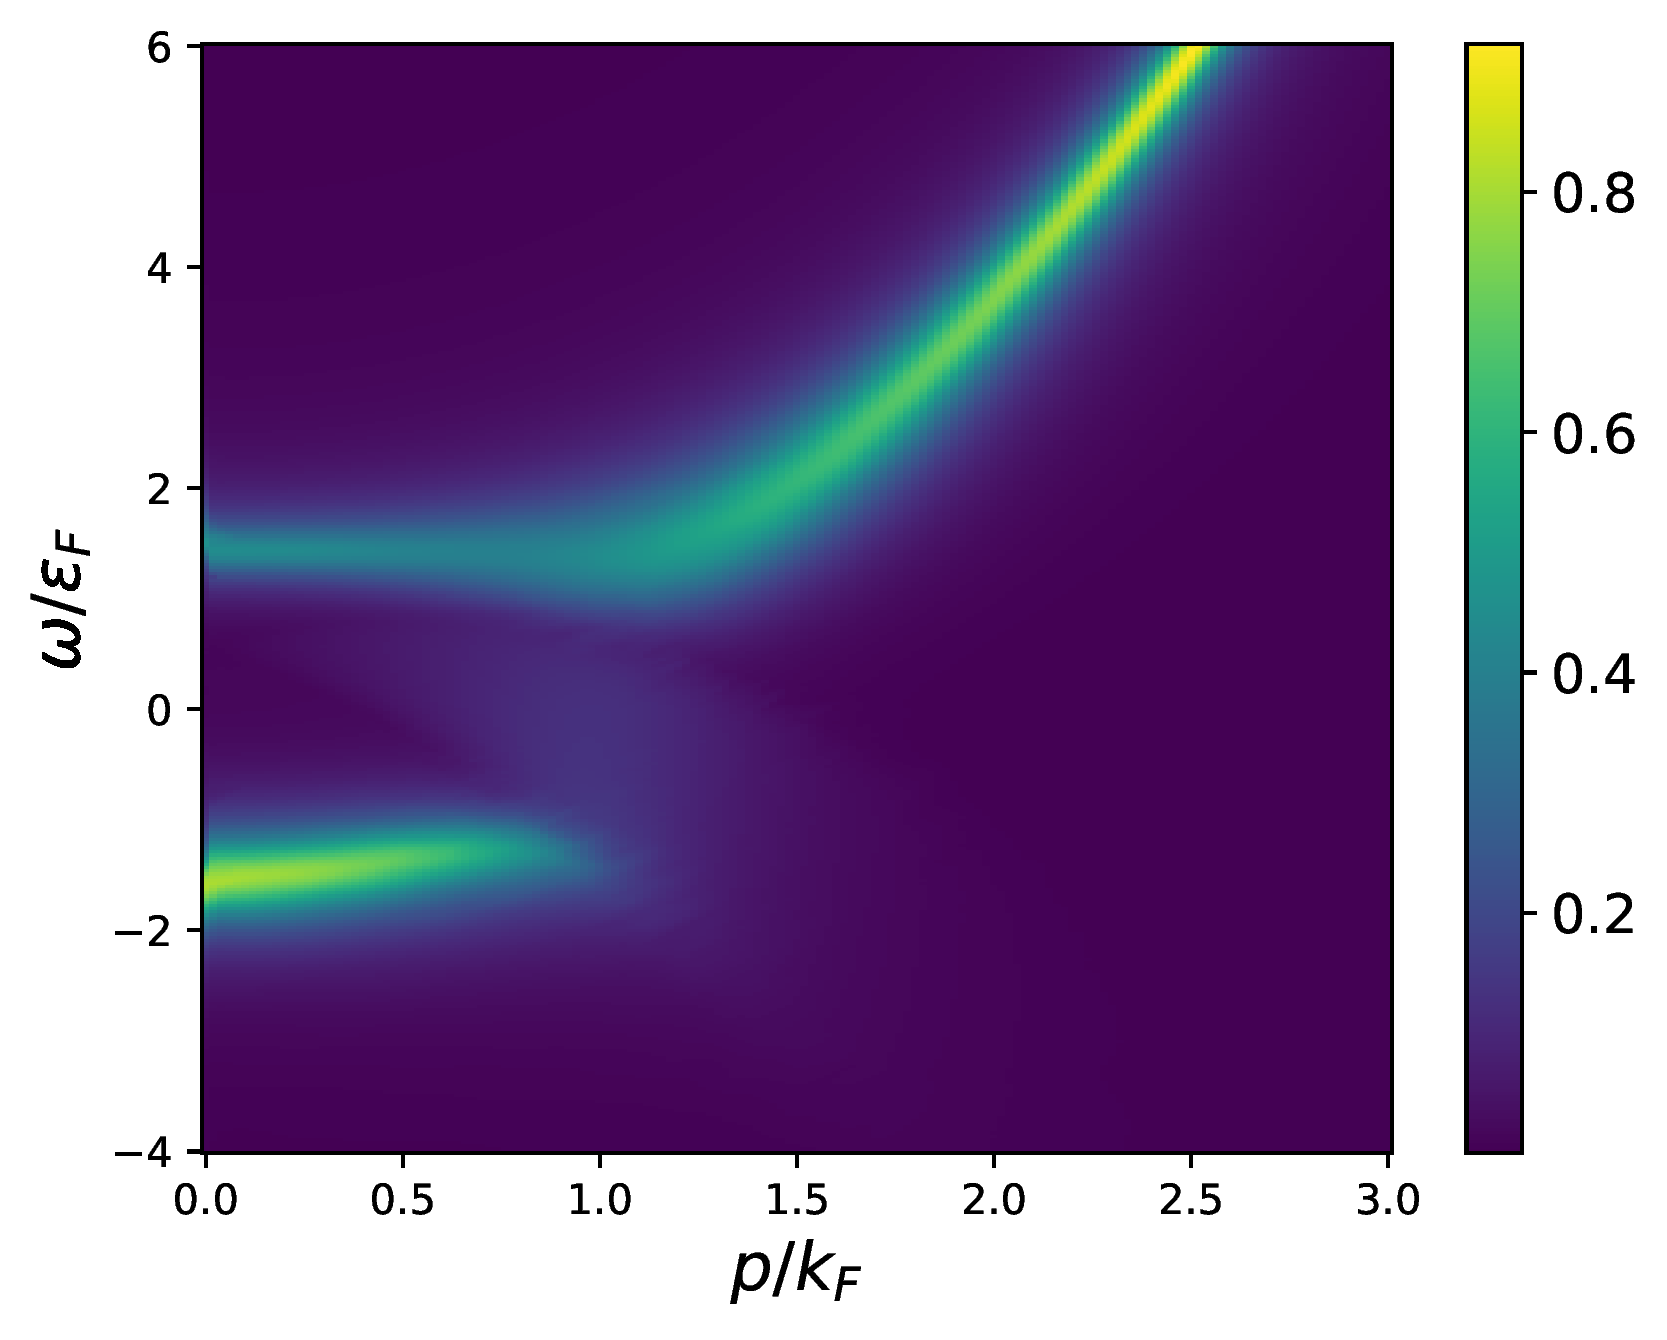
\includegraphics[width=0.401\textwidth]{figs/fermion_T=0.2_iter=8.png}}
	\caption[Fermion spectral functions close to the critical temperature]{Iterations of the fermionic spectral function $\rho_{\psi}\,\varepsilon_F$ at unitarity for $\beta\mu=2$.}
	\label{fig:fermion-specs-critical}
\end{figure*}
%
\begin{figure*}[t]
	\centering
	\subfigure[Iteration 7]{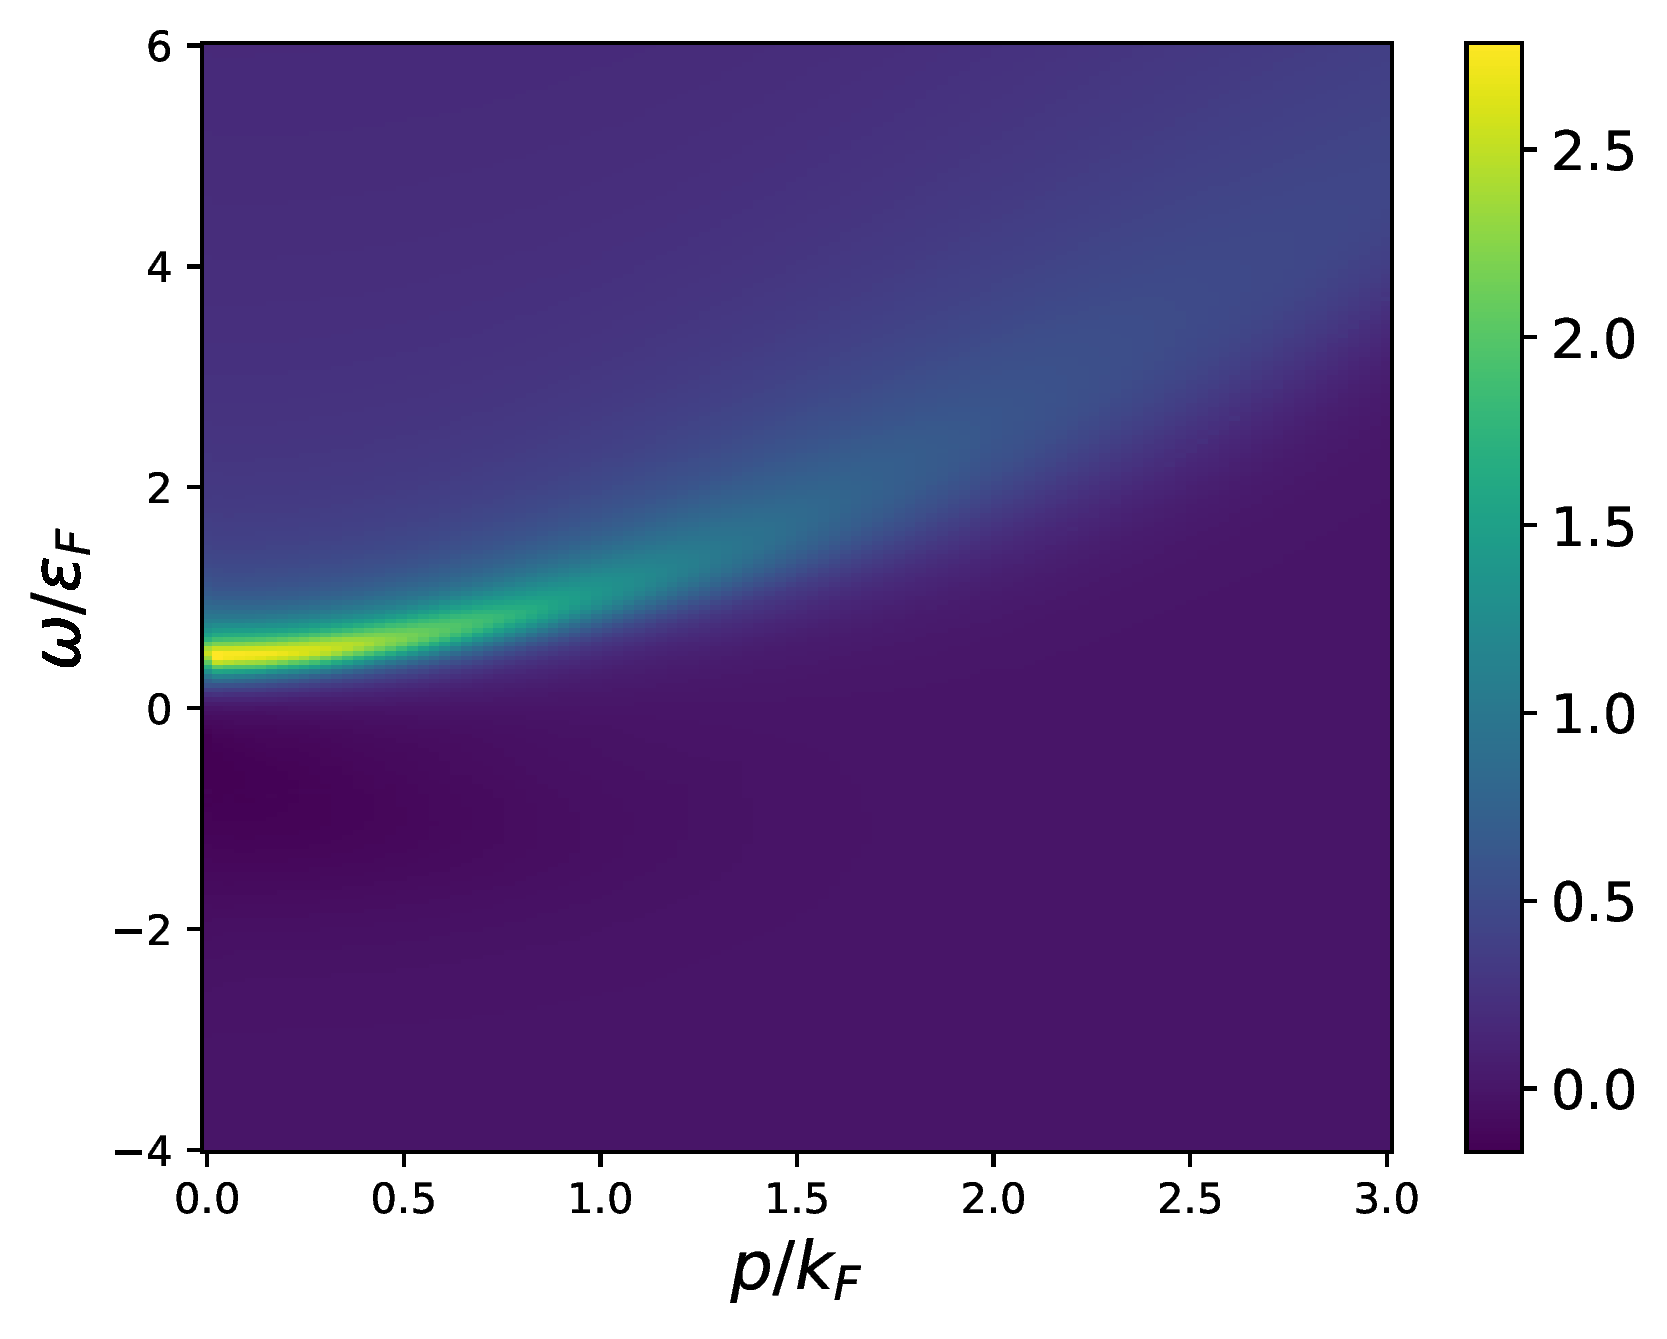
\includegraphics[width=0.392\textwidth]{figs/boson_T=0.2_iter=7.png}}
	\subfigure[Iteration 8]{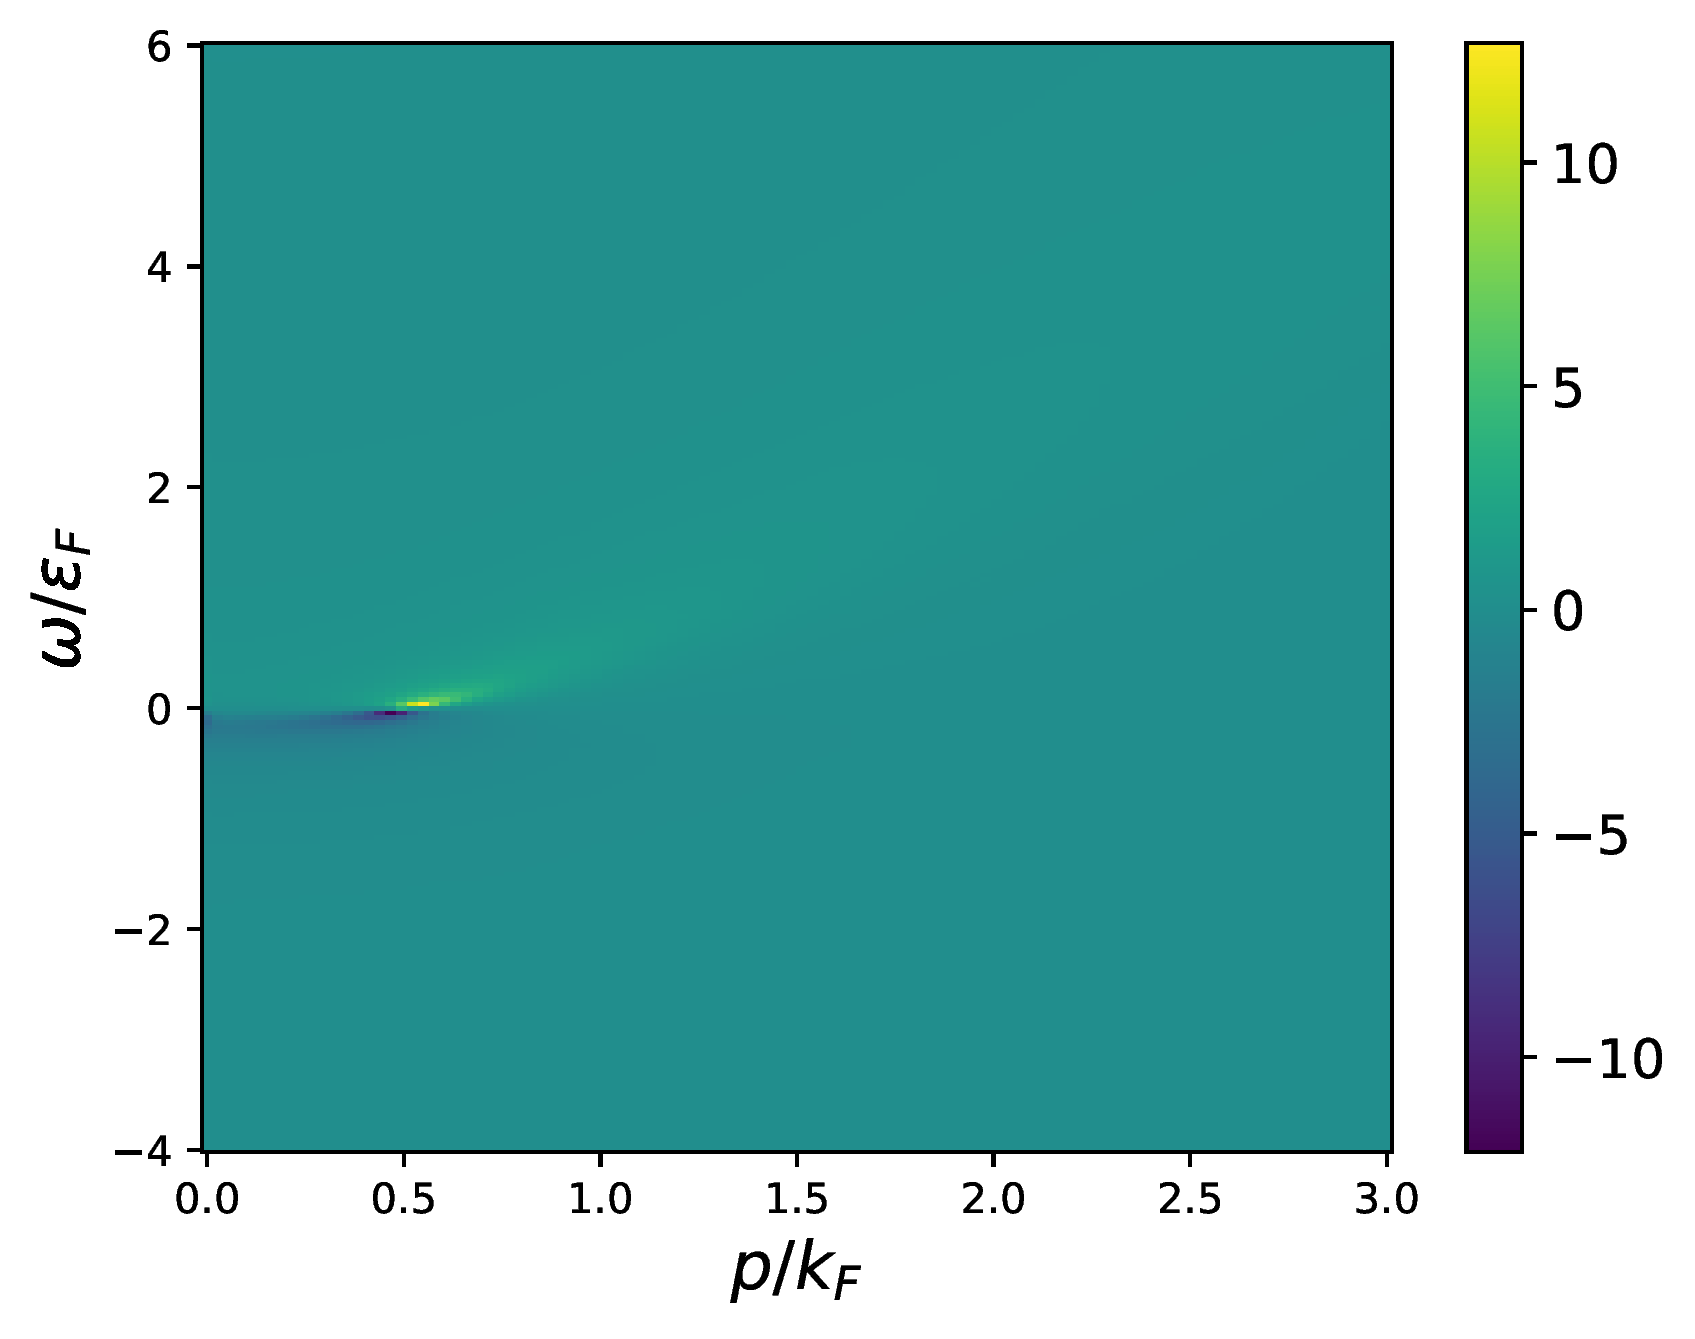
\includegraphics[width=0.397\textwidth]{figs/boson_T=0.2_iter=8.png}}
	\caption[Boson spectral functions close to the critical temperature]{Iterations of the bosonic dimer spectral function $h^2\rho_{\phi}\,\varepsilon_F/(8\pi)$ for $\beta\mu=2$.}
	\label{fig:boson-specs-critical}
\end{figure*}

As a consequence, the boson spectral function reveals crucial information about the critical region of the phase transition to the superfluid state. It is well-known that the onset of superfluidity is marked by the divergence of the boson propagator at zero frequency and momentum $G^{-1}_{\phi}(0,\bm{0})=0$. This property is known as the Thouless criterion~\cite{Thouless1960}. Thus, the closer and sharper the peak gets at the origin, the closer the system is to the phase transition, until the spectral function eventually diverges at the critical temperature.

\newpage

In order to evaluate spectral functions in the symmetry-broken phase, one has to ensure that the Thouless criterion~\cite{Thouless1960} is fulfilled, i.e. the bosons have to be gapless. At the same time, the gap parameter $\Delta$ has to be updated selfconsistently. This is a challenging numerical task and could not be implemented in the framework of this Thesis. There are many approaches and approximations to determine the gap parameter~\cite{Haussmann2009,Perali2004}. One way might be to choose $\Delta$ and a modified interaction strength such that the Thouless criterion is fulfilled~\cite{Haussmann2009,Lang2023}. Non-selfconsistent results in the broken phase can be obtained easily from the mean-field treatment presented in Section~\ref{section:nambu-gorkov-formalism}. The anomalous fermion spectral function is already well-known in the literature, see also~\cite{Bzdusek2013}. However, the bosonic anomalous spectral function is barely discussed. First non-selfconsistent considerations are presented in~\cite{Pieri2004-1}, however a selfconsistent treatment is absent and remains the subject for future work. We leave this as an exercise for the reader.

As an outlook for future work, one might also consider the mass and spin-imbalanced case, see~\cite{Punk2007,Punk2010,Frank2018}. In the following, we will use the spectral functions to calculate physical observables and benchmark our results against existing data.


\newpage


%%%%%%%%%%%%%%%%%%%%%%%%%%%%
\subsection*{Radio-frequency spectroscopy}
\label{section:rf-spectra}

From the calculated spectral functions, it is possible to obtain the experimentally measurable radio-frequency (rf) spectra~\cite{Punk2007,Schneider2009}. In this part, we apply our numerical framework at unitarity to describe the recent experimental data from MIT~\cite{Mukherjee2019}. For the computation of rf spectra $I(\omega)$ from the fermion spectral functions $\rho_{\psi}$, we take the formula~\cite{Haussmann2009}
%
\begin{align}
	\label{eq:rf-spectra}
	I(\omega) = \int_{\bm{q}} \rho_{\psi}(\varepsilon_{\bm{q}}-\omega-\mu,\bm{q})\, n_F(\varepsilon_{\bm{q}}-\omega-\mu) \,.
\end{align}
%
Note that the chemical potential $\mu(T)$ is temperature-dependent and has to be determined selfconsistently from the number equation~\eqref{eq:density}. More explicitly, the number density $n=1/(3\pi^2)$ is fixed by the choice $k_F=1$ and temperature is measured in units of $T_F$. Consequently, the chemical potential $\mu(T)$ has to be chosen such that the density stays constant~\cite{Tajima2019}. It is easy to see that the rf spectrum is normalized to the density $n$~\cite{Haussmann2009},
%
\begin{align}
	\label{eq:rf-dens}
	n = 2\int_{-\infty}^{\infty} d\lambda\, I(\lambda) \,.
\end{align}
%

\begin{figure}[htb]
	\begin{minipage}[t]{.492\textwidth}
		\centering
		\subfigure[]{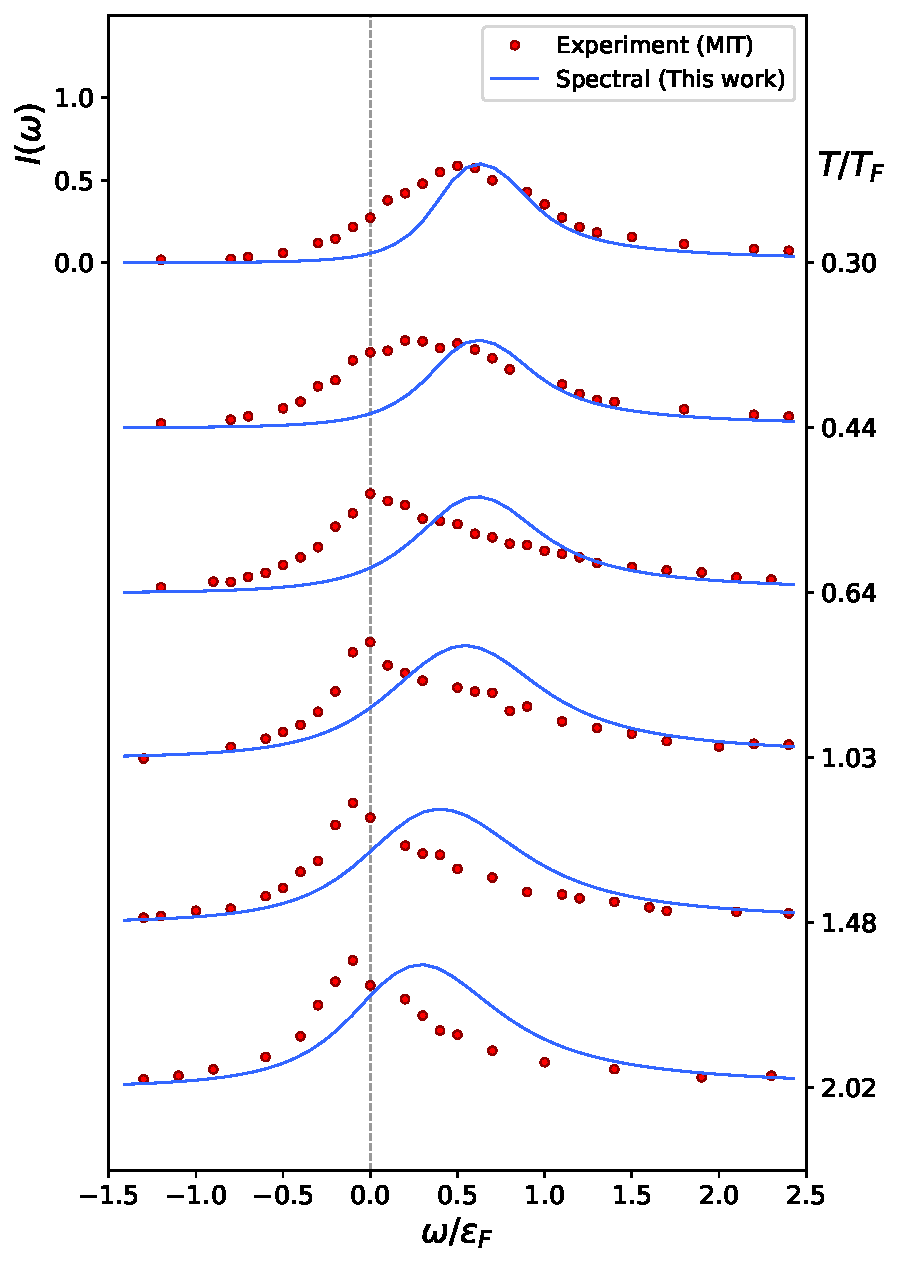
\includegraphics[width=\textwidth]{figs/rf_spectra.pdf}}
	\end{minipage}
	\hfill
	\begin{minipage}[t]{.49\textwidth}
		\centering
		\subfigure[]{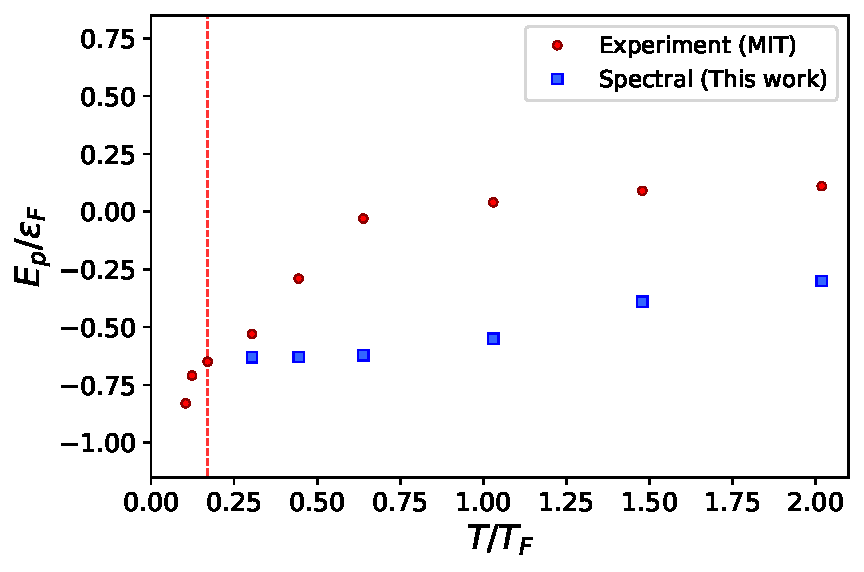
\includegraphics[width=0.95\textwidth]{figs/peak.pdf}}
		\raggedleft
		\subfigure[]{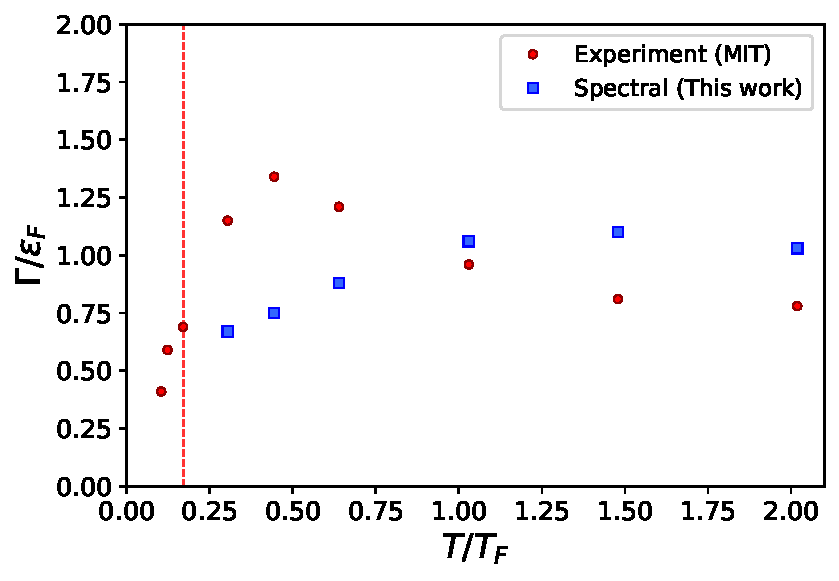
\includegraphics[width=0.92\textwidth]{figs/lifetime.pdf}}
	\end{minipage}
	\caption[Rf spectra of the unitary Fermi gas]{(a) Calculated ejection rf spectra $I(\omega)$ for the spin-balanced unitary Fermi gas as a function of the reduced temperature $T/T_F$. Results of this work (solid lines) are compared to experimental data from MIT~\cite{Mukherjee2019} (points). A Fourier broadening of $0.1\varepsilon_F$ to account for the finite experimental resolution, and a right-shift by $0.09\varepsilon_F$ to account for the final state interaction were applied. (b) Peak position ($E_p=-\hbar\omega$) and (c) full width at half maximum $\Gamma$ extracted from the rf spectra. The red vertical dashed line in (b) and (c) marks the superfluid phase transition.}
	\label{fig:rf-spectra}
\end{figure}

Fig.~\ref{fig:rf-spectra} shows our results in comparison with the experimental data from MIT~\cite{Mukherjee2019}. Apart from adjusting the peak heights, no fitting parameter have been used. In order to account for the finite rectangular rf pulse duration and, thus, a finite experimental resolution, the calculated spectra have to be convolved with $\mathrm{sinc}^2(\omega T/2)$, where $T$ is the rf pulse duration~\cite{Haussmann2009}. Additionally, the curves have to be right-shifted by an amount of $0.09\varepsilon_F$ to eliminate the residual final state effect~\cite{Hu2022}. Even after taking into account all these possible factors, the calculated rf spectra do not fit the experimental data for higher temperatures very well. This was also observed in~\cite{Hu2022} for the case of a highly spin-imbalanced unitary Fermi gas. A possible explanation might be the absence of a trap average, see e.g.~\cite{Schmidt2012}, since the trap potential is not ideally box shaped.


%%%%%%%%%%%%%%%%%%%%%%%%%%%%
\subsection*{Tan contact} \label{sec:contact}

Another test of the calculated spectral functions is the determination of the momentum-dependent occupation number $n(p)$ and Tans contact $C$~\cite{Rossi2018,Jensen2020}. The contact $C$ can be calculated in many different ways~\cite{Hu2011,Palestini2010}. One way is via the large frequency behavior of the rf spectrum $I(\omega)$~\cite{Haussmann2009,Schneider2009}
%
\begin{align}
	\label{eq:rf-contact}
	\lim_{\omega\rightarrow\infty} I(\omega) = \frac{C}{2\sqrt{2}\pi^2}\,\omega^{-3/2} \,.
\end{align}
%
Another direct way is via the imaginary-time boson propagator $G_{\phi}(\tau,\bm{x})$~\cite{Rossi2018}
%
\begin{align}
	\label{eq:vertex-contact}
	C = -G_{\phi}(\tau=0^-,\bm{x}=\bm{0}) \,,
\end{align}
%
which is used by imaginary-time computations like the Luttinger-Ward approach~\cite{Frank2018}. In this work, we extract the contact via the large momentum behavior of the occupation number $n(p)$~\cite{Boettcher2012, Hu2011}
%
\begin{align}
	\label{eq:contact}
	n(p) = \int_{\lambda} \rho_{\psi}(\lambda,\bm{p})\, n_F(\lambda) \,, \qquad \lim_{p\rightarrow\infty} n(p) = \frac{C}{p^4} \,.
\end{align}
%

\begin{figure}[h]
	\centering
	\subfigure[$\beta\mu=-0.5$]{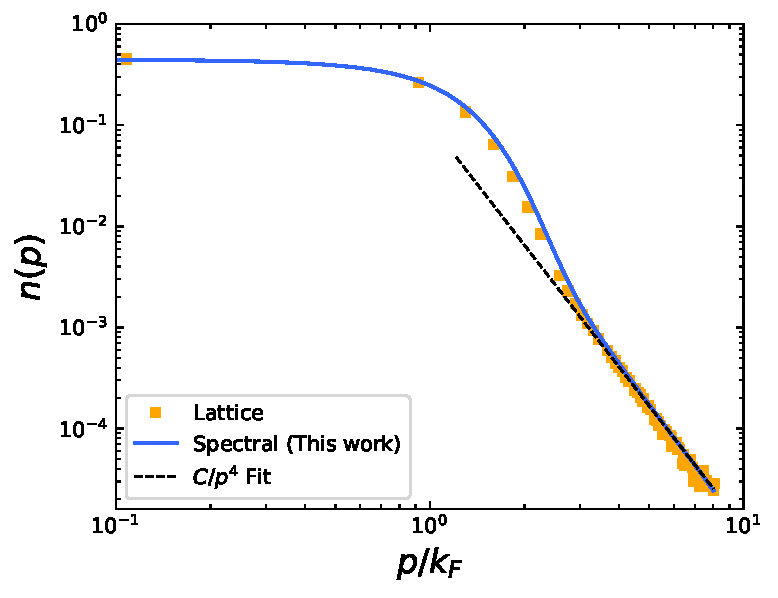
\includegraphics[width=0.47\textwidth]{figs/momentum_density_lattice_n05.pdf}}
	\subfigure[$\beta\mu=0.5$]{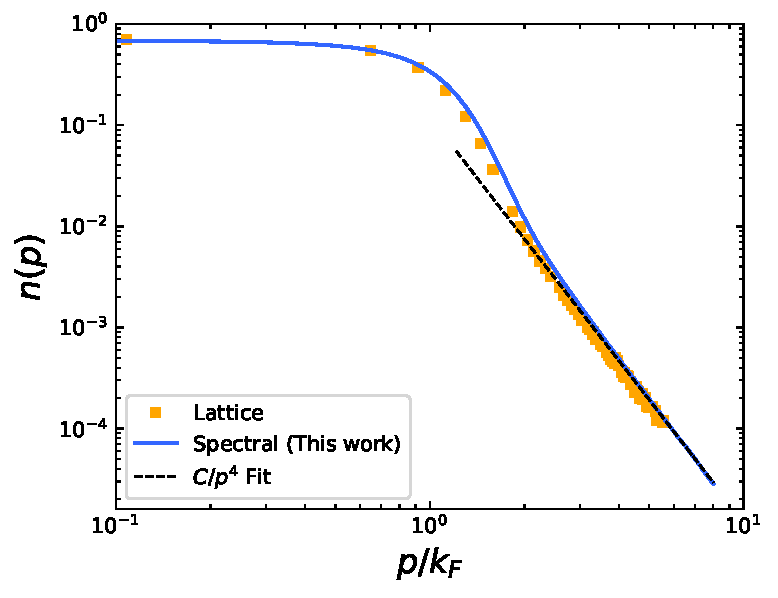
\includegraphics[width=0.47\textwidth]{figs/momentum_density_lattice_05.pdf}}
	\caption[Momentum distribution $n(p)$]{Large $p$ behavior of the occupation number $n(p)$. Results of this work are compared to lattice Monte Carlo data from~\cite{Bauer2023}.}
	\label{fig:momentum-density}
\end{figure}

\begin{figure}[t]
	\centering
	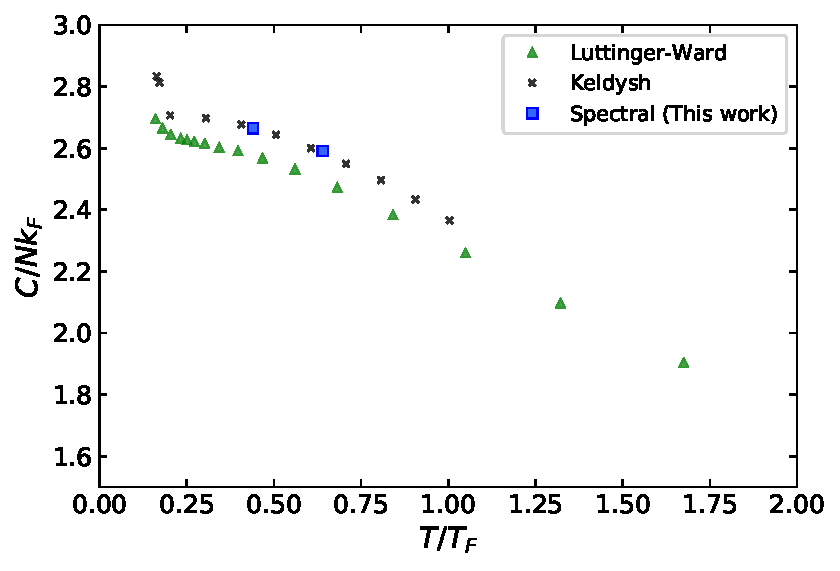
\includegraphics[width=0.67\linewidth]{figs/contact.pdf}
	\caption[Contact $C/Nk_F$ of the unitary Fermi gas]{Dimensionless contact $C/Nk_F$ of the spin-balanced unitary Fermi gas as a function of the reduced temperature $T/T_F$. Results of this work are compared to the Luttinger-Ward approach in imaginary-time~\cite{Frank2018} and another real-time approach using the Keldysh formalism~\cite{Lang2023}. The contact from the real-time approaches was obtained from the large momentum tail $n(k)=C/k^4$.}
	\label{fig:contact}
\end{figure}

Fig.~\ref{fig:contact} shows results for the Tan contact obtained with the spectral approach in comparison with the Luttinger-Ward~\cite{Frank2018} and Keldysh~\cite{Lang2023} approach. We note that the contact of the imaginary-time Luttinger-Ward method was determined directly from the boson propagator, while the contact of the real-time approaches was calculated from the large momentum behavior of the occupation number. Thus, these results are not directly comparable since the imaginary-time results are obtained with a different method. However, both real-time approaches seem to yield the same results.

Additionally, we show the momentum density distribution functions $n(p)$ in a double logarithmic plot for different $\beta\mu$ in Fig.~\ref{fig:momentum-density}. The $1/p^4$ tail for $p\gg k_F$ is clearly visible. We show lattice Monte Carlo results of Marc Bauer from our group for comparison. In the simulations, a lattice size of $13^3$ spatial points and 160 imaginary-time steps is used~\cite{Bauer2023}. In agreement with other works, the contact from selfconsistent T-matrix approaches seems to be slightly larger than experimental data or lattice Monte Carlo results~\cite{Mukherjee2019}. Thus, it is not surprising that the large momentum tail of our results is slightly above the lattice data.


%%%%%%%%%%%%%%%%%%%%%%%%%%%%
\subsection*{Density equation of state} \label{sec:density_eos}

The last benchmark of the calculated spectral functions is the density equation of state. Thermodynamic quantities, such as the total particle density, can be calculated precisely in Euclidean frequencies without the need of analytic continuation. For this reason, it is a good way to validate the new spectral approach against well tested and robust imaginary-time calculations. 

The total density $n$ of fermions at finite chemical potential $\mu$ and temperature $T$ can be calculated from the spectral function via~\cite{Schneider2009}
%
\begin{align} \label{eq:density}
	n = 2\,T\sum_{\omega_n}\int_{\bm{p}}G_{\psi}(\omega_n,\bm{p}) = 2\int_{\lambda,\bm{p}}\rho_{\psi}(\lambda,\bm{p})\,n_F(\lambda) \,.
\end{align}
%
Fig.~\ref{fig:density_eos} shows the results for the normalized density $n/n_0$ as a function of dimensionless chemical potential $\beta\mu$ in comparison with all other available approaches. The density $n_0$ of the non-interacting Fermi gas is given by $n_0=2\int_{\bm{p}}n_F(p^2-\mu)=-2\mathrm{Li}_{3/2}(-e^{\beta\mu})/\lambda_T^3$, where $\lambda_T=\sqrt{4\pi/T}$ is the thermal wavelength and $\mathrm{Li}_{3/2}$ is a polylogarithm function~\cite{Abramowitz1972}.

In the calculation of the density through the spectral function, the high momentum tail can not be neglected. If the numerical spectral function is given on a finite grid with momentum cutoff $\Lambda\gg k_F$, the contribution from outside the grid follows with~\eqref{eq:contact},
%
\begin{align}
	\delta n_{>\Lambda} = 2 \int_{\Lambda}^{\infty}\frac{d^3p}{(2\pi)^3} \frac{C}{p^4} = \frac{C}{\pi^2\Lambda} \,,
\end{align}
where $C$ is the contact introduced before. Note that this estimation is only valid when the numerical cutoff $\Lambda$ is chosen large enough, such that the asymptotic behavior set in already. Then one can extrapolate the large $p$ region and take its contribution into account. Fig.~\ref{fig:momentum-density} shows that our numerics reproduce the asymptotic $1/p^4$ tail very well for $p\approx 8k_F$ already. The missing contribution from the high momentum tail is around $10\%$.

It is important to note that our real-time method reproduces the results of the well tested Luttinger-Ward approach~\cite{Haussmann2007,Frank2018}. Moreover, the other real-time approach based on the Keldysh formalism agrees very well with our results. This agreement is crucial since all methods build on the same underlying theory and resummation of diagrams.


\begin{figure}[t]
	\centering
	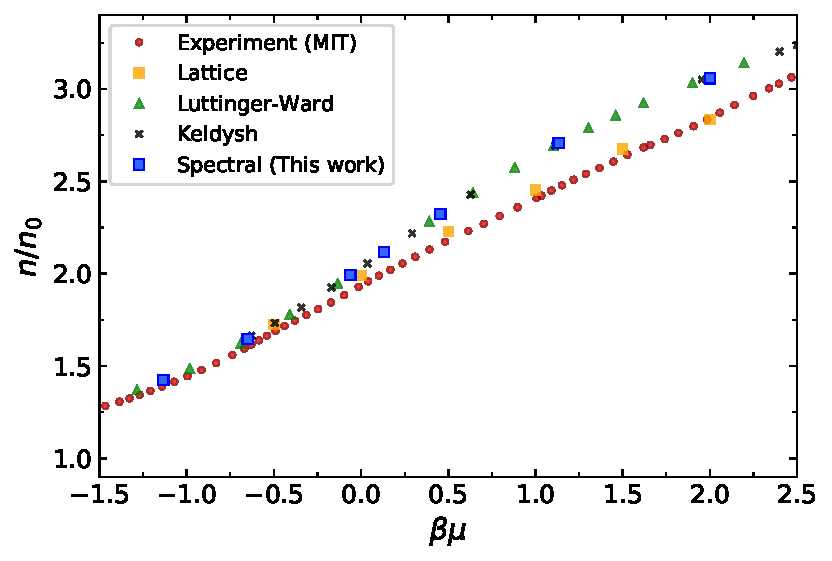
\includegraphics[width=0.67\linewidth]{figs/density_eos.pdf}
	\caption[Density equation of state of the unitary Fermi gas]{Normalized density $n/n_0$ of the spin-balanced unitary Fermi gas as a function of dimensionless chemical potential $\beta\mu$. Results directly obtained in real frequencies (this work) in comparison with experimental data from MIT~\cite{Ku2012}, lattice Monte Carlo data from~\cite{Bauer2023}, Luttinger-Ward results~\cite{Haussmann2007} and another real-time approach based on the Keldysh formalism~\cite{Lang2023}.}
	\label{fig:density_eos}
\end{figure}
